\chapter{A transport model for hard partons in the QGP}
\label{chapter:transport}
Hard partons are predominately created in perturbative scatterings at the earliest stage of relativistic heavy-ion collisions.
The distribution of the hard partons gets modified by the medium, and the final distribution carries information about the medium, as well as the hard-soft interaction properties.

Among the many ways of describing the in-medium evolution of hard partons, 
the transport approach has a unique advantage. 
Here, we refer to the transport approach as a class of models that evolve the semi-classical particle distribution function of hard partons in real-time.
Transport models can often be formulated as particle-level simulations, which provide easy coupling to local properties of a dynamically evolving and fluctuating medium, and an exclusive final state.
Of course, challenges exist when applying transport models to high energy collisions.

First, there are different assumptions of the interactions between the hard partons and the medium to be made.
Two commonly assumed extremes are:
\begin{itemize}
\item[1] A weakly coupled picture: the medium consists of perturbative quasi-particles (scattering centers) whose distribution is close to local thermal equilibrium.
Hard partons scatter perturbatively with these well-separated scattering centers. A Boltzmann equation describes its dynamics.
\item[2] Diffusion picture: interactions between the medium and the hard parton are frequent and soft, and there are substantial many-body and non-perturbative effects. Such dynamics are solved using a Langevin equation, and a drag and a diffusion coefficient model the effect of these soft interactions on the hard parton. 
\end{itemize}
These two commonly used approaches are not necessarily mutually exclusive and can have an overlapping range of validity. 
For example, the effect of soft momentum exchange processes in the perturbative calculation can be very well modeled by a diffusion equation \cite{Ghiglieri:2015ala,Dai:2019hbi}.
These different assumptions on the interaction between the medium and the hard probe are primarily due to our inadequate theoretical tools in describing the QGP medium in the strongly coupled regime.
On the one hand, this becomes an uncertainty intrinsic to the transport approach, until one finds a convincing way of calculating the dynamics of the strongly coupled QGP medium from first principles.
On the other hand, experiments may be able to tell which assumption (or a combination of both) is preferred and answer the very question of how the sQGP participates in the jet-medium interactions.

A second difficulty is that a semi-classical transport equation is inadequate in treating quantum coherence.
Indeed, a quantum transition will always be bounded by the uncertainty principle: a process with momentum scale $Q$ can not be localized within a space-time extent of $1/Q$.
While in the semi-classical transport model, one always specifies a local point in space-time where the interaction takes place.
This is valid if the momentum scale $Q$ is high enough that $1/Q$ is much smaller than the resolution of the transport model, e.g., characterized by the mean-free-path in the Boltzmann equation.
However, the soft and collinear divergences of QCD bremsstrahlung (or more generally, parton branching and merging) processes generate an abundance of small-$Q$ events whose spatial extent can be much greater than the mean free path, which happens for both the vacuum parton shower and the medium-induced parton shower in certain phase space regions.
For medium-induced branching, this is the QCD analog of the Landau-Pomeranchuk-Migdal (LPM) effect \cite{PhysRev.103.1811,Wang:1994fx,Zakharov:1996fv}, and the radiation pattern is changed qualitatively.
When this happens, strictly speaking, the semi-classical transport equation is not the appropriate tool.
However, considering the advantages of the transport formulation, we want to develop a minimum set of modification to the semi-classical transport that can mimic the quantum effects of medium-induced branchings approximately.

We start by introducing a class of widely used transport equations: the (linearized) Boltzmann equation and the Langevin equation.
Then, we combine these two approaches into a hybrid one by introducing a cut-off distinguishing hard and soft momentum transfer processes and build the transport model in the incoherent limit.
After that, we provide a brief review of the theory of QCD in-medium parton branching processes at leading order, discussing its various approximations and also the numerical solutions in a simplified medium.
With these theoretical insights, the primary outcome of this chapter is developing a ``modified Boltzmann'' transport approach, treating the medium-induced parton branching with an approximate LPM effect.
Finally, the simulations of the transport model are compared to theoretical expectations to validate the implementation in different regimes.
We will show that the modified transport approach can reasonably describe the energy spectrum of the medium-induced splitting vertex for different channels $q\rightarrow q+g$, $g\rightarrow g+g$ and $g\rightarrow q+\bar{q}$.
Treatment of the heavy quark masses effect and running coupling are also investigated.
For future references, in the very end, we make comparisons between two other Monte-Carlo approaches for medium-induced radiation with the present one and comment on potential problems.

\section{The Boltzmann equation}
The Boltzmann equation evolves the particles' distribution function under the effect of localized collisions. 
By localization, it means that the time scale of the collision has to be much smaller than the mean free-path $\tau \ll \lambda$. 
Therefore, the collision probability can be evaluated using a local particle distribution function.
It also allows one to include only few-body collision processes, because the probability of interacting with an additional particle during this collision is small $P \approx \tau/\lambda \ll 1$.
At weak coupling, we will see in the next section that this is indeed the case for elastic collisions or soft and large-angle radiation. 
However, for radiation with a large formation time, the process becomes ``non-local''.
Accordingly, the Boltzmann formulation needs to be modified quite fundamentally for such processes.
In this section, we only focus on local interactions.

With two-body to two-body (elastic) and two-body to three-body (inelastic, including the reverse process) processes, the Boltzmann equation for particle specie $a$ takes the following form,
\begin{eqnarray}
\frac{\partial f^a}{\partial t} + \vec{v}\cdot\frac{\partial f^a}{\partial \vec{x}} + \frac{\partial E}{\partial \vec{x}}\cdot\frac{\partial f^{a}}{\partial \vec{p}} = - \sum_{b,c,d}\mathcal{C}_a^{a+b\leftrightarrow c+d}- \sum_{b,c,d,e}\mathcal{C}_a^{a+b\leftrightarrow c+d+e}
\end{eqnarray}
On the left hand side, the distribution function $f^{a}(t, \vec{x}, p)$ undergoes transport with velocity $\vec{v} = \partial E/\partial \vec{p}$, and a potential force $\vec{f} = -\partial E/\partial \vec{x}$.
On the right-hand side of the equation, the $2\leftrightarrow 2$ and $2\leftrightarrow 3$ collision terms are functionals of the distribution functions.
The summation of $b,c,d,e$ iterates over all other particle species including $a$.
Using the elastic process as an example and neglecting degeneracy of the internal quantum number for simplicity, the collision term can be separated into gain and loss terms,
\begin{eqnarray}
\mathcal{C} &=& \mathcal{C}_\textrm{loss} + \mathcal{C}_\textrm{gain}\\
&=& \int_{bcd} f^a(p_1)f^b(p_2)[1+\epsilon^c f^c(p_3)][1+\epsilon^d f^d(p_4)] \overline{|M|^2}(p_1, p_2; p_3, p_4) \\\nonumber
&-& \int_{bcd} f^c(p_3)f^d(p_4)[1+\epsilon^a f^a(p_1)][1+\epsilon^b f^b(p_2)] \overline{|M|^2}(p_3, p_4; p_1, p_2) \\
&=& \int_{bcd} \left\{
f^a(p_1)f^b(p_2)[1+\epsilon^c f^c(p_3)][1+\epsilon^d f^d(p_4)] \right. \label{eq:collision-term:symmetry} \\\nonumber
&& \left.- f^c(p_3)f^d(p_4)[1+\epsilon^a f^a(p_1)][1+\epsilon^b f^b(p_2)]\right\}
\overline{|M|^2},
\end{eqnarray}
where the crossing symmetry of the matrix-elements has been used in the last line of the equation ($\overline{|M|^2}(p_1^a, p_2^b; p_3^c, p_4^d) = \overline{|M|^2}(p_3^c, p_4^d; p_1^a, p_2^b) = \overline{|M|^2}$), and the phase-space integral is 
\begin{eqnarray}
\int_{bcd} = \prod_{i\in {b,c,d}}\int\frac{dp_i^3}{2E_i (2\pi)^3} (2\pi)^4 \delta^{4}(p_a+p_b - p_c-p_d).
\end{eqnarray}
The $\epsilon = 0, -1, 1$ corresponds to classical, Fermi-Dirac, and Bose-Einstein statistics depending on the nature of the particle.
The first term in the integration represents the loss of a particle of type ``$a$'' in the phase-space around the point $(x, p_1)$ due to elastic collision, and the second term represents the gain of a particle of type ``$a$'' due to the reverse process.
The symmetry in the microscopic matrix-element is essential for the kinetic equation to satisfy detailed balance: the probability to transition from one microscopic state to anther equals that of the reverse process.
The detailed balance ensures the thermal equilibrium limit of the system. 
Assume the system evolves long enough in a box of finite volume and there is no spatial variance of the distribution function.
Then the left side of equation \ref{eq:collision-term:symmetry} is zero, and the static solution has to satisfy the relation,
\begin{eqnarray}
f^a f^b (1+\epsilon f^c) (1+\epsilon f^d) = f^c f^d (1+\epsilon f^a) (1+\epsilon f^b),
\end{eqnarray}
for the entire phase-space and every combination of particle species.
Therefore, the following combination is conserved for each reaction channel.
 \begin{eqnarray}
\frac{f^a}{(1+\epsilon^a f^a)} \frac{f^b}{(1+\epsilon^b f^b)}
= \frac{f^c}{(1+\epsilon^c f^c)} \frac{f^d}{(1+\epsilon^d f^d)}
\end{eqnarray}
The available conservation quantities are the four-momentum; therefore, one solution to the previous equation is,
\begin{eqnarray}
\frac{f^a}{(1+\epsilon^a f^a)} = e^{-\beta \mu_a-\beta p\cdot u}
\end{eqnarray}
for every particle species with parameters $\mu, \beta$ and a four vector $u$ ($u^2 = 1$). 
So the static solution of the distribution is 
\begin{eqnarray}
f^a(p) = \frac{1}{ e^{\beta \mu_a+\beta p\cdot u} - \epsilon^a} \label{eq:thermal}\\
\mu_a +\mu_b = \mu_c + \mu_d \label{eq:chem}
\end{eqnarray}
The fist line is the distribution function in thermal (kinetic) equilibrium, and the second line is the requirement for reaching chemical equilibrium. 
One can identify the $\beta$ and $\mu$ parameter as the inverse temperature and chemical potential. The $u$ vector is the flow velocity of the cell as can be seen from the average velocity,
\begin{eqnarray}
\left\langle \frac{p^\mu}{M} \right\rangle = \frac{\int f(p) \frac{p^\mu}{M} dp^3}{\int f(p) dp^3} = \frac{\int f(p) \frac{p^\mu}{M} dp^3}{\int f(p) dp^3} = u^\mu
\end{eqnarray}

\subsection{The linearized Boltzmann equation and the diffusion limit}
Analytic solutions of the Boltzmann equations are almost impossible; even numerical solutions and simulations are highly non-trivial tasks.
However, under certain circumstances, a linearization of the Boltzmann equation is possible and greatly simplifies both the analytic analysis as well as the numerical implementation.

Hard particles (jet partons, heavy flavors) either have a large momentum $p\gg T$ or a large mass $M \gg T$. 
In heavy-ion collisions, the hard cross-section drops fast with the increase of $p_T$ and $m_T$, so hard partons are very rare in an actual event and the occupation number of hard partons is small $f_H \ll 1$.
Therefore, one can neglect the quantum statistics terms in the Boltzmann equation for them $1+\epsilon f_H \approx 1$.
Also, the collision terms with more than one uncorrelated hard particle in the initial state can also be neglected since these contributions are proportional to $f_H^2 \ll f_H$. 
Finally, we also assume that the response of the bulk of the particles to the hard particles is small, and shall neglect any collision terms that involve a hard parton in the Boltzmann equation for the bulk distribution function\footnote{\singlespacing recently studies show that such back reactions are important for the study of full jet observables \cite{PhysRevC.99.054911}, but we only consider leading particles in this thesis}.
Under these approximations, one arrived at a set of equations that are linearized with respect to the hard parton:
\begin{eqnarray}
\frac{df_H}{dt} &=& -\mathcal{C}_H[f_H, f_{\textrm{bulk}}], \label{eq:hard-bulk-eq}\\
\frac{df_{\textrm{bulk}}}{dt} &=& -\mathcal{C}[f_{\textrm{bulk}}].
\end{eqnarray}
The collision term $\mathcal{C}_H$ is a linear operator on $f_H$.

For the medium particles, the equations are still complicated.
However, by observing that the time it takes for the low momentum bulk particles to reach local thermalization is much shorter than the relaxation time of the hard particles, a zeroth-order approximation would be using the local thermal distribution \ref{eq:thermal}.
The space-time evolution of the temperature $T$, chemical potential $\mu$ and flow velocity $u$ can be obtained from a hydrodynamic simulation.
Replacing the medium distribution function by the thermal one in equation \ref{eq:hard-bulk-eq}, one arrives at a closed and linearized equation for the hard particles.
Here we write down the equations assuming both classical statistics and the conservation of the hard parton's species, and only the elastic collision terms are shown for simplicity,
\begin{eqnarray}
\frac{df^H}{dt} &=& -\sum_{b} \int_{234} \left\{
f^H(p_1)f^b_{eq}(p_2) - f^H(p_3)f^b_{eq}(p_4)\right\}
\overline{|M|^2} \\
&=& - \int \left\{
f^H(p_1) w(p_1; p_3) - f^H(p_3) w(p_3, p_1)\right\}\frac{dp_3^3}{2E_3 (2\pi)^3}.
\end{eqnarray}
The $w(p; p')$ is the transition probability density for a particle with momentum $p$ into momentum state $p'$,
\begin{eqnarray}
w(p; p') = \sum_b\int_{24} f_{eq}^b(p_2) \overline{|M|^2}(p, p_2; p', p_4)
\end{eqnarray}

Using local thermal solutions for the bulk particles is a strong assumption. 
The degree of local thermalization in realistic events is still an open question, especially at the early stage of the heavy-ion collision. 
Moreover, whether the system can be understood in terms of quasi-particle degrees of freedom is a different question.
In an extreme weakly coupled system $g\ll 1$, one expects that the pressure and energy density can be explained using fundamental degrees of freedom: quarks and gluons, with perturbative corrections \cite{Blaizot:2000fc,Strickland:2010tm,Su:2015esa}.
However, with a large $g$ estimated from phenomenological studies, such a perturbative description may not be the most efficient way of understanding the bulk medium, and non-perturbative physics can play an essential role. 
Interpreting the medium in terms of microscopic degrees-of-freedom seem to be an unavoidable step of the Boltzmann equations; however, it is possible to ``integrate out'' the microscopic details in the soft limit of interaction into a set of transport coefficients.

\paragraph{The Fokker Planck equation}
In the soft-momentum transfer $q = p'-p$ limit  $|q| \ll |p|$, one can expand the collision term to second-order in $q$, and the linearized Boltzmann equation reduces to the Fokker-Planck type of equation,
\begin{eqnarray}
\frac{df}{dt} &=& - \int \left\{
f(p) - \left[f(p) +  \vec{q}\frac{\partial f}{\partial\vec{p}} + \frac{1}{2}\vec{q}\vec{q}\frac{\partial^2 f}{\partial\vec{p} \partial\vec{p}} \right]
\right\} w(p',p)\frac{dp_3^3}{2E_3 (2\pi)^3} \\
&=& - \int \left\{ \vec{q}\frac{\partial f}{\partial\vec{p}} - \frac{1}{2}\vec{q}\vec{q}\frac{\partial^2 f}{\partial\vec{p} \partial\vec{p}}
\right\} w(p',p)\frac{dp_3^3}{2E_3 (2\pi)^3} \\
&=&  -\eta_D(p) \frac{\partial f}{\partial\vec{p}} + \frac{1}{2}B(p)\frac{\partial^2 f}{\partial\vec{p} \partial\vec{p}},
\end{eqnarray}
where the vector function $A$ and tensor function $B$ are the first- and second-order moments of the transition rate,
\begin{eqnarray}
A_i(p) &=& \int w(p,p+q) q_i \frac{dp_3^3}{2E_3 (2\pi)^3},\\
B_{ij}(p) &=& \int w(p,p+q) q_i q_j \frac{dp_3^3}{2E_3 (2\pi)^3}.
\end{eqnarray}
One remark is that although the form of the Fokker-Planck equation can be derived as the soft limit of the linearized Boltzmann equation, its range of applicability is different from the latter.
It is because the transport coefficients are well defined in general, regardless of whether one assumes quasi-particle type microscopic dynamics.
Therefore in our model, we replace the soft sector of the Boltzmann equation with the Fokker-Planck equation so that the use of ``medium quasi-particles'' is restricted to hard momentum transfer processes.

Moments beyond second order are neglected in deriving the Fokker-Planck equation. 
This truncation is justified if the interaction is frequent enough so that within the smallest time scale that is concerned, a statistical description of the effect of many interactions in terms of the first (mean) and the second moments (variance) is adequate.
However, if the physical processes are rare, fluctuations contained in higher moments are indispensable and a diffusion equation is not a good approximation.

\paragraph{Transport coefficients and the Einstein relation} 
The $A$ and $B$ functions have to satisfy certain symmetries, as the only special direction after averaging over medium effects is the direction of motion.
Therefore,  $\vec{A} = \eta_D \vec{p}$ defines the drag coefficient  $\eta_D$; the tensor $B$ can be decomposed into a transverse part and a longitudinal part, with the respective momentum diffusion coefficients $\kappa$ and $\kappa_L$,
\begin{eqnarray}
B_{ij} = \kappa_L \frac{p_i p_j}{p^2} + \kappa \left(\delta_{ij} - \frac{p_i p_j}{p^2}\right).
\end{eqnarray}

One notices that the medium temperature does not show up explicitly in the Fokker-Planck equation,
\begin{eqnarray}
\frac{df}{dt} = \frac{\partial}{\partial p_i}\left(\eta_D p_i + \frac{1}{2}\frac{\partial}{\partial p_j} B_{ij}\right)f.
\end{eqnarray}
To guarantee the system has a thermalized solution, $A$, $\Kpara$ and $\Kperp$ are not independent.
Given a static and homogeneous medium at equilibrium with temperature $T$, $f = N\exp\left(-\beta E\right)$, the equation reduces to
\begin{eqnarray}
0 &=& \ppi(\phi p_i f)\\
\phi &=& \eta_D - \frac{\Kpara}{2TE} + \frac{\partial \Kpara}{\partial p^2} + \frac{\Kpara-\Kperp}{p^2}.
\end{eqnarray}
The Einstein relation $\phi = 0$ guarantees the existence of an equilibrium solution,
\begin{eqnarray}
\eta_D = \frac{\Kpara}{2TE} - \frac{\partial \Kpara}{\partial p^2} - \frac{\Kpara-\Kperp}{p^2}
\label{eq:ein-rel}
\end{eqnarray}
This is where the temperature shows up explicitly in the Fokker-Planck equation.

\section{Hard parton transport in the incoherent limit}
In this section, we proceed to use a local and incoherent calculation of hard parton scatterings and will defer a detailed discussion on the inclusion of the LPM effect to the next section.
The partonic processes are categorized into elastic (particle number conserving) and inelastic processes (particle number non-conserving). 
The inelastic processes are further divided into parton-splitting and parton-fusing contributions. 

\subsection{Hard/soft separation: elastic collisions}
In a quasi-particle picture of the QGP, the hard parton collides with medium partons and transfers a certain amount of four-momentum.
These processes can be computed at leading order in the weakly coupled theory, where the collision cross-section is calculated using the dressed gluon propagator inside the medium \cite{PhysRevD.44.1298},
\begin{eqnarray}
D^{\mu\nu}(\omega, k) = \frac{\delta^{\mu 0}\delta^{\nu 0}}{k^2 - \Pi_L(\omega, k)} + \frac{\hat{P}_T^{\mu\nu}}{\omega^2 - k^2 - \Pi_T(\omega, k)}
\end{eqnarray}
where $\Pi_T$ and $\Pi_L$ are the self energies for the transverse and longitudinal modes.
Due to the presence of the medium, the dressed propagator loses its Lorentz invariance and depends on the complicated functions $\Pi_T$ and $\Pi_L$.
The resulting cross-section formula will be equally complicated.
Fortunately, it has been shown recently in \cite{Ghiglieri:2015ala} that simplification is possible at leading order in rewriting the elastic processes as large-angle scattering and small-angle diffusion.
In such an approach, one chooses a scale $Q_\textrm{cut}$ with a formal range of $gT \ll Q_\textrm{cut} \ll T$.
For processes with momentum transfer to the medium larger than the cut-off  (hard modes), the medium screening effect is neglected and we use matrix-elements in the vacuum.
While for processes smaller than the cut-off (soft-mode), the propagator receives significant contributions from the screen effect.
The soft processes happen frequently and only involve small momentum transfers, satisfying the requirements of diffusion approximation.
This separation allows the following modeling of the elastic interaction between hard partons and the medium,
\begin{eqnarray}
\frac{df}{dt} = \mathcal{D}(Q_{\textrm{cut}})[f] + \mathcal{C}^{2\leftrightarrow 2}(Q_{\textrm{cut}})[f].
\end{eqnarray}
Here, particles are continuously evolved by the diffusion process with their momenta occasionally changed by large-$Q$ scatterings.
Later we will verify that the cut-off dependence in the diffusion and scattering component indeed cancels for ``physical observations'' at a sufficiently small coupling.
However, the phenomenological value of $g$ is very large so that the residue cut-off dependence may be significant. 
The advantage of the current formulation is that a diffusion process can also model certain non-perturbative effects with an additional contribution to the transport coefficient.

\paragraph{Transport coefficients for soft modes} The transverse and longitudinal transport parameters below the cut-off have been calculated in \cite{Ghiglieri:2015ala},
\begin{eqnarray}
\hat{q}_S &=& \int dq^2 \frac{\alpha_s m_D^2 T}{q^2 (q^2+m_D^2)} = g^2 C_R T m_D^2  \ln\left(1+\frac{Q_{\textrm{cut}}^2}{m_D^2}\right).
\label{eq:qS} \\
\hat{q}_{S,L} &=& \int dq^2 \frac{\alpha_s m_\infty^2 T}{q^2 (q^2+m_\infty^2)} = g^2 C_R T m_\infty^2  \ln\left(1+\frac{Q_{\textrm{cut}}^2}{m_\infty^2}\right)
\label{eq:qSL} 
\end{eqnarray}
$m_\infty^2 = m_D^2/2$ is the thermal mass of the gluon. 
The drag force is determined by the Einstein relation in equation \ref{eq:ein-rel},
\begin{eqnarray}
\eta_D = \frac{\hat{q}_{S,L}}{2ET} - \frac{d\hat{q}_{S,L}}{dp^2} - \frac{2\hat{q}_{S,L} - 2\hat{q}_S}{2p^2}
\end{eqnarray}

\paragraph{Scattering rate for hard modes} For the large-$Q$ $2\rightarrow 2$ scattering processes, the collision rates are computed by integrating the vacuum matrix-element, 
\begin{eqnarray}
R = \frac{d}{2E_1}\int  \frac{d^3p_2}{2E_2(2\pi)^3} f_0(p_2)2\hat{s} \int_{-\hat{s}}^{Q_{\textrm{cut}^2}}\frac{d\sigma}{d\hat{t}}d\hat{t}
\end{eqnarray}
The integration is restricted to large momentum transfers above $Q_{\textrm{cut}}$, and therefore we do not impose additional screening effects to regulate the matrix-element.
In this work, the $2\rightarrow 2$ matrix-element only includes the $\hat{t}$-channel contribution.

\subsection{Hard/soft separation: inelastic collisions}
Similarly, incoherent inelastic processes are divided into small-$Q$ diffusion induced radiation/absorption ($1\leftrightarrow 2$), and large-$Q$ $2\leftrightarrow 3$ processes.

\paragraph{Diffusion induced branching} For the incoherent diffusion-induced splitting rate, we borrow the expression from \cite{Cao:2017hhk} while stripping the time-dependent phase factor,
\begin{eqnarray}
R_{1\rightarrow 2} = \int d k_\perp^2 dx \frac{\alpha_s P(x) \hat{q}_S(Q_{\textrm{cut}})}{2\pi (k_\perp^2 + m_\infty^2)^2}
\end{eqnarray}
where a gluon thermal mass is added to screen the divergence.
Because these gluons are induced by processes with medium momentum transfer below the cut-off, $Q_{\textrm{cut}}$ appears in the formula.
For the reverse $2\rightarrow 1$ processes, a similar reaction rate can be written down,
\begin{eqnarray}
R_{2\rightarrow 1} = \int e^{-\beta \omega} d k_\perp^2 dx \frac{\alpha_s P(x) \hat{q}_S(Q_{\textrm{cut}})}{2\pi (k_\perp^2 + m_\infty^2)^2}.
\end{eqnarray}
$\omega$ is the thermal parton's energy, and $x$ is defined as the fraction of the thermal parton's energy to that of the final state hard parton.
These specific expressions are associated to the medium rest frame.

\paragraph{Large-$Q$ $2\leftrightarrow 3$ process} 
Regarding the $2\rightarrow 3$ matrix-element, in a previous study \cite{Ke:2018tsh}, we used to employ an improved version of the original Gunion-Bertsch cross-section that works under the limits $k_\perp, q_\perp \ll \sqrt{s}$ and $x q_\perp \ll k_\perp$ \cite{PhysRevD.25.746,Fochler:2013epa,Uphoff:2014hza}.
In the present study, we keep improving the matrix-elements by following the derivation in \cite{Fochler:2013epa} while relaxing the condition $x q_\perp \ll k_\perp$.
Therefore the updated matrix-elements contain the correct vacuum splitting function in the collinear limit.
We summarize the matrix-elements here and have attached a derivation in appendix \ref{app:ME},
\begin{eqnarray}
\overline{|M^2|}_{g+i\rightarrow g+g+i} &=& \overline{|M^2|}_{g+i\rightarrow g+i} P_{gg}^{g(0)}  D_{gg}^{g},\\
\overline{|M^2|}_{g+i\rightarrow q+\bar{q}+i} &=& \frac{C_F d_F}{C_A d_A}\overline{|M^2|}_{g+i\rightarrow g+i} P_{q\bar{q}}^{g(0)} D_{q\bar{q}}^{g,}\\
\overline{|M^2|}_{q+i\rightarrow q+g+i} &=& \overline{|M^2|}_{q+i\rightarrow q+i} P_{qg}^{q(0)} D_{qg}^{q}.
\end{eqnarray}
Index $i$ represents a quark, an antiquark or a gluon.
The two body matrix-elements that enter the $2\rightarrow 3$ matrix-element are always required to be the $t$-channel contribution.
$P_{bc}^{a(0)}(x)$ are vacuum splitting functions from parton $a$ to partons $b$ and $c$,
\begin{eqnarray}
P_{gg}^{g(0)}  &=& g^2  C_A\frac{1+x^4+(1-x)^4}{x(1-x)},\\
P_{qg}^{q(0)} &=& g^2  C_F\frac{1+(1-x)^4}{x},\\
P_{q\bar{q}}^{g(0)} &=& g^2  \frac{N_f}{2}\left(x^2+(1-x)^4\right).
\end{eqnarray}
The $D_{bc}^{a}$ contains the interference structure,
\begin{eqnarray}
D_{qq}^{g} &=& 
C_A(\vec{a}-\vec{b})^2 + C_A(\vec{a}-\vec{b})^2 \\\nonumber
&-& C_A (\vec{a}-\vec{b})\cdot (\vec{a}-\vec{c}),
\\
D_{q\bar{q}}^{g} &=& 
C_F(\vec{a}-\vec{b})^2 + C_F(\vec{a}-\vec{b})^2 \\\nonumber
&-& (2C_F-C_A) (\vec{a}-\vec{b})\cdot (\vec{a}-\vec{b}),
\\
D_{qg}^{q} &=& 
C_F(\vec{c}-\vec{a})^2 + C_F(\vec{c}-\vec{b})^2 \\\nonumber
&-& (2C_F-C_A) (\vec{c}-\vec{a})\cdot (\vec{c}-\vec{b}).
\end{eqnarray}
with the vectors given by
\begin{eqnarray}
\vec{a} = \frac{\vec{k}_\perp - x\vec{q}_\perp}{(\vec{k}_\perp - x\vec{q}_\perp)^2},
\vec{b} = \frac{\vec{k}_\perp - \vec{q}_\perp}{(\vec{k}_\perp - \vec{q}_\perp)^2},
\vec{c} =  \frac{\vec{k}_\perp}{\vec{k}_\perp^2}.
\end{eqnarray}

\subsection{The final incoherent transport equation and Monte-Carlo technique}
Combining all these processes, we summarize the incoherent linearized-Boltzmann plus Langevin equation:
\begin{eqnarray}
\frac{df}{dt} = \mathcal{D}[f] + \mathcal{C}_{1\leftrightarrow 2}[f] + \mathcal{C}_{2\leftrightarrow 2}[f] + \mathcal{C}_{2\leftrightarrow 3}[f].
\end{eqnarray}
The distribution function undergoes soft diffusion and diffusion induced-radiation. 
Hard collisions with the medium are included as $2\leftrightarrow 2$ and $2\leftrightarrow 3$ collision terms.
The next section is devoted to the inclusion of the LPM effect to such an incoherent transport equation.
We now discuss the numerical techniques for simulating the above equation.

The Monte Carlo method starts from representing the distribution function by an ensemble of particle states,
\begin{eqnarray}
f(t,x,p) \approx \sum_{i} \delta^3(x-x_i(t)) \delta^3(p-p_i(t))
\end{eqnarray}
For linearized transport equations, it is sufficient to consider the dynamics of one such particle.
Within a short time step $\Delta t$, a particle undergoes scattering with a certain probability.
In between subsequent collisions, the particle propagates with drag force and the random thermal force.

\paragraph{Order of operation} In the presence of two types of operation: collision $\mathcal{C}[f_Q]$ and diffusion $\mathcal{D}[f_Q]$:
\begin{eqnarray}
\nonumber
  \frac{df}{dt}  &=& 
\left( \mathcal{\hat{C}} + \mathcal{\hat{D}} \right) f_Q.
\end{eqnarray}
In principle, the order of operations on the particle should matter.
However, a different choice of ordering only results in an $O(\Delta t^2)$ change in the updated distribution function.
It is evident with the formal solution of the equation,
\begin{eqnarray}
\nonumber
f_Q(x,p) &=& \exp\left\{ \int_{x'}^x \gamma u \cdot dx \left( \mathcal{\hat{C}} + \mathcal{\hat{D}} \right) \right\} f_Q(x',p)\\
&\approx & e^{\Delta t \hat{C}}e^{\Delta t \hat{D}} f_Q(x', p) + \mathcal{O}(\Delta t^2)
\end{eqnarray}

\paragraph{The diffusion solver}
The Fokker Planck equation can be solved as an ensemble of particles governed by Langevin dynamics.
The Langevin equation in the post-point discretization scheme is \cite{He:2013zua},
\begin{eqnarray}
\Delta \vec{x}_i &=& \frac{p}{E}\Delta t\\
\Delta \vec{p}_i &=& -\Gamma \vec{p}_i \Delta t + \sqrt{\tensor{B}(p+\Delta p) \Delta t  }\vec{\xi}
\end{eqnarray}
$\Gamma$ is the Langevin drag term, and $\vec{\xi}$ is a unit-variance Gaussian random force.
$\tensor{B} = \Ppara \Kpara + \Pperp \Kperp$ are the diffusion coefficients in the tensor form.
$\Ppara$ and $\Pperp$ project any vector into the direction parallel and perpendicular to the direction of motion.

The diffusion coefficients are directly related to the one in the Fokker Planck equation $\Kpara = \hat{q}_L$, and $\Kperp = \hat{q}/2$.
While the relation between the drag coefficient in the Fokker Planck equation $\eta_D$ and the drag force $\Gamma$ in the Langevin equation is discretization scheme dependent.
In the post-step scheme, this relation is \cite{He:2013zua},
\begin{eqnarray}
p_j \Gamma  = p_jA + \left(\sqrt{\Kpara}\Ppara_{lk} + \sqrt{\Kperp}\Pperp_{lk}\right) \ppl \left( \sqrt{\Kpara}\Ppara_{kj} + \sqrt{\Kperp}\Pperp_{kh} \right).
\end{eqnarray}
and reduces to,
\begin{eqnarray}
\Gamma &=& \eta_D + \frac{d \Kpara}{dp^2} + \frac{2\sqrt{\Kpara\Kperp} - 2\Kperp}{p^2} \\
 &=& \frac{\Kpara}{2TE} - \frac{1}{p^2}\left( \sqrt{\Kpara} - \sqrt{\Kperp} \right)^2.
\end{eqnarray}
The Einstein relation between $\eta_D$ and diffusion coefficient is used in the last step.

\paragraph{The scattering solver}
For two-body scattering, neglecting quantum statistics, the collision rate in the rest frame of the medium is,
\begin{eqnarray}
R_a(p) = \sum_{b,c,d}\frac{1}{2E_a}\int \frac{dp_b^3}{(2\pi)^3 2E_b} f_0(p_b) \int d\Phi_m |M^2|_{ab\rightarrow cd}
\end{eqnarray}
A similar expression can also be obtained for $2\leftrightarrow 3$ processes.
For a short amount of time $\Delta t$, the probability to have no collision is $P_{0} = \exp(-\Delta t R)$.
The number of multiple independent collisions satisfies a Poisson distribution with mean $N = \Delta t R$. 
For a particle-based simulation, one always needs to ensure that $\Delta t$ is small enough $(\Delta t \ll 1/R)$ so that effectively there is at most one collision happening within the time step.
Once a collision is sampled to happen, the full final state can be obtained by further sampling each scattering channel and the momentum phase-space differential rates.

The multi-dimensional phase-space sampling is performed sequentially for the initial state and final state phase-space.
For $2\rightarrow 2$ and $2\rightarrow 3$ body processes, we rewrite the integrated rate in the fluid cell rest frame as,
\begin{eqnarray}
R_{2m}(E_1, T) &=& \frac{d}{\nu} \frac{1}{2E_1}\int \frac{e^{-\beta E_2}dp_2^3}{(2\pi)^32E_2} 
\int d\Phi_m\overline{|M|^2}.
\end{eqnarray}
If vacuum matrix-elements are used, the nested integration is a Lorentz invariant quantity, and we can choose to calculate it in the center-of-mass frame of the two-body collision, 
\begin{eqnarray}
\int d\Phi_m\overline{|M_{22}|^2} &=& 2E_12E_2v_{\textrm{rel}}\sigma \nonumber \\
 &=& 2(s-M^2)\sigma_{\textrm{CoM}}^{22}(\sqrt{s}, T)\nonumber \\
  &=& F_{2m}(\sqrt{s}, T)
\end{eqnarray}
where $\sigma$ is the cross-section of the process.
In practice, we tabulate the values of the integrated rates and cross-sections. 
The sampling of initial state $p_2$ determines the center-of-mass energy of the process $s = (p_1+p_2)^2 = 2(E_1 E_2 - p_1p_2 \cos\theta_{12})$.
Subsequently, we sample the momentum-transfer $q$-differential cross-section with $\sqrt{s}, T$ as inputs, and reconstruct the final states given the initial state and $q$.

The sampling of the $3\rightarrow 2$ body process is more difficult due to the larger number of parameters to specify the initial state kinematics,
\begin{eqnarray}
R_{32}(E_1, T) = \frac{d}{\nu} \int \frac{e^{-\beta E_2}dp_2^3}{(2\pi)^32E_2} \frac{e^{-\beta k}dk^3}{(2\pi)^32k}
\int d\Phi_2\overline{|M|^2}.
\end{eqnarray}
The Lorentz invariant nested integral is a function of the initial state 3-body kinematics and temperature,
\begin{eqnarray}
\int d\Phi_2\overline{|M|^2} = F_{32}(\sqrt{s}, \sqrt{s_{12}}, \sqrt{s_{1k}}, T),
\end{eqnarray}
where $s = (p_1+p_2+k)^2$ is the center of mass energy, $s_{12} = (p_1+p_2)^2$ and $s_{1k} = (p_1+k)^2$.
It requires a four-dimensional table for the value of $F_{32}$ and a five-dimensional initial state sampling.
The tabulation of a high-dimensional rate and cross-section tables is manageable if a proper approximating function $A(x, y, \cdots)$ is proposed that captures the limiting behavior of the target function $T(x, y, \cdots)$.
Then, tabulating the ratio of $T/A$ would be extremely efficient and accurate with a moderate-size table.

The sequential sampling breaks the original $m+n$ body phase-space sampling into two lower-dimensional samplings.
However, as one should notice, the prerequisite is that we rewrite the integration over the final state momentum of the matrix-element into a Lorentz invariant form; therefore, the table only depends on the Mandelstam variables and temperature.
This appealing feature is broken by the inclusion of either
quantum statistics or in-medium propagators in the matrix-elements. 
Because quantum statistics introduces factors like $1\pm f(p\cdot u)$ to the final momentum integral and the in-medium propagator is not Lorentz invariant, resulting in a $F_{nm}$ that depends on the relative velocity between the collision system and the medium rest frame.
The result is a significant increase in the dimensionality and complexity of the problem. 
Fortunately, the separation of hard and soft modes allows one to use vacuum matrix-elements at large momentum transfer and absorbs the reference frame dependence into the diffusion equation, which is much easier to solve.

\section{The Landau-Pomeranchuk-Migdal effect: theory}
\begin{figure}
\singlespacing
\centering
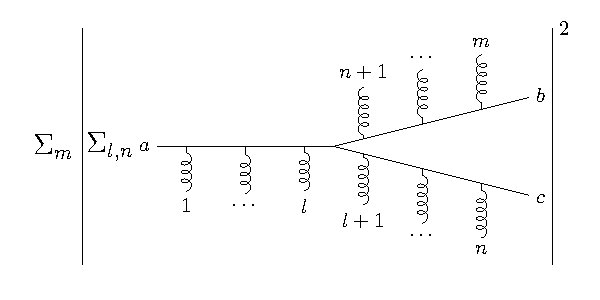
\includegraphics[width=.8\textwidth]{splitting.pdf}
\caption[A schematic demonstration of the physics of in-medium parton]{A schematic demonstration of the physics of in-medium parton bremsstrahlung. The hard parton ``$a$'' splits into two hard partons ``$b$'' and ``$c$''. The hard partons (quarks or gluon) are denoted as straight lines. The hard system constantly interacts with the medium through gluon exchanges, denoted as the loop lines. One sums the squared amplitudes ($|\cdots|^2$) over an arbitrary number ($m$) of interactions with the medium. Each amplitude has to include all the interference contribution.
Finally, one does an ensemble average over the medium configurations.}
\label{fig:split}
\end{figure}
In the last section, all the processes are treated as instantaneous; however, a process takes a finite amount of time for its final states to lose coherence. 
For elastic collisions, this time is $1/m_D \sim 1/gT$ which is still short compared to the mean-free-path $\lambda \sim 1/g^2 T$, provided a sufficiently small $g$.
For inelastic process, the light-cone energy difference between the initial and final states is,
\begin{eqnarray}
\delta E = \frac{k_\perp^2}{2k} + \frac{p_\perp^2}{2p} - \frac{{p'}_\perp^2}{2{p'}} = \frac{ [(1-x)\vec{k}_\perp - x\vec{p}_\perp]^2}{2x(1-x)E}
\end{eqnarray}
By the uncertainty principle, the coherence time for such a transition is on the order of $\tau_f = 1/\delta E$, termed the ``formation time'' of the radiation. 
In this region of phase space $k_\perp^2, p_\perp^2 < g^2x(1-x)ET$, the average number of collisions during the radiation becomes a relatively large number $N = \tau_f/\lambda >1$, so the picture of induced-radiation from independent scattering centers breaks down.
It has been shown that these multiple scatterings should be resummed \cite{Zakharov:1996fv,Zakharov:1997uu,Baier:1996kr} (please refer to figure \ref{fig:split} for a schematic demonstration), and the leading order resummed radiation probability is,
\begin{eqnarray}
\frac{dP^{a}_{bc}}{d\omega} &=& \frac{\alpha_s P^{0,a}_{bc}(x)}{x^2(1-x)^2 E^2}\mathfrak{Re}\int_0^\infty dt_1 \int_{t_1}^{\infty} dt_2\\\nonumber &&\nabla_{\mathbf{b}_1} \cdot\nabla_{\mathbf{b}_2} \left\{G(t_2, \mathbf{b}_2; t_1, \mathbf{b}_1) - G_0(t_2, \mathbf{b}_2; t_1, \mathbf{b}_1) \right\}|_{\mathbf{b}_1, \mathbf{b}_2 \rightarrow 0}
\label{eq:theory-dR}
\end{eqnarray}
$P^{0,a}_{bc}(x)$ is the vacuum splitting function, and $x$ is the energy fraction carried by the daughter $b$.
Inside the double-time integral, $G$ is the propagator of the following Hamiltonian for the transverse dynamics of the splitting system,
\begin{eqnarray}
\hat{H} &=& \frac{-\nabla^2_{\mathbf{b}} + m^2_\textrm{eff}}{2x(1-x)E} - i \Gamma_3(\mathbf{b})\\
\Gamma_3(\mathbf{b}) &=& \frac{C_a-C_b+C_c}{2}\Gamma_2(\mathbf{b}) + \frac{C_a-C_c+C_b}{2}\Gamma_2(x\mathbf{b}) \\\nonumber
&&+ \frac{C_b+C_c-C_a}{2}\Gamma_2((1-x)\mathbf{b}),
\end{eqnarray}
and $G_0$ is the free propagator. 
The variable $\mathbf{b}$ is the Fourier transformation dual of the transverse momentum, and is usually referred to as the impact-parameter (not to be confused with the one used in the nuclear collision geometry).
$m^2_\textrm{eff}$ is a combination of both parton bare masses and thermal masses.
Finally, the interaction $\Gamma_3(\mathbf{b})$ encodes the transverse broadening of the three body system $a\rightarrow b+c$ \cite{Zakharov:1997uu}.
It has three two-body contributions $\Gamma_2(\mathbf{b})$.
The vacuum piece $G_0$ is subtracted from $G$ so that this formula only computes the medium-induced radiation.
The two gradient operators at time $t_1$ and $t_2$ come from the action of the radiation vertices, meaning this transition receives coherence contribution from $t_1$ to $t_2$.
If one neglects the mass term and rewrites $G$ as $G_0 -i G_0\Gamma_3 G$, the equation simplifies to 
\begin{eqnarray}
\nonumber
\frac{dP^{a}_{bc}}{d\omega} &=& \frac{\alpha_s P^{0,a}_{bc}(x)}{x^2(1-x)^2 E^2}\mathfrak{Re}\int_0^\infty dt_1 \int_{t_1}^{\infty} dt_2\\ &&\nabla_{\mathbf{b}_1} \cdot\nabla_{\mathbf{b}_2} [G_0(-i\Gamma_3) G](t_2, \mathbf{b}_2;t_1, \mathbf{b}_1)|_{\mathbf{b}_1, \mathbf{b}_2 \rightarrow 0},\\
&=& \frac{\alpha_s P^{0,a}_{bc}(x)}{x^2(1-x)^2 E^2}\mathfrak{Re}\int_0^\infty dt_1 \int_{t_1}^{\infty} dt_2 F(t_2; t_1).
\end{eqnarray}
$F(t_2, t_1)$ is a short notation for the term to be integrated.

The interaction potential $\Gamma_2(\mathbf{b})$ depends on the assumption of the probe-medium interaction.
For example, in a weakly coupled theory, a compact result is obtained at leading order \cite{Aurenche:2002pd},
\begin{eqnarray}
\Gamma_2(\mathbf{b}) = \frac{1}{\pi}\int \frac{d\mathbf{q}_\perp^2}{(2\pi)^2} \frac{g^2 T m_D^2 (1-e^{i\mathbf{b}\cdot\mathbf{q_\perp}})}{q_\perp^2(q_\perp^2+m_D^2)}
\end{eqnarray}

There are two systematic ways to investigate equation \ref{eq:theory-dR}.
In a method called the opacity expansion \cite{Wiedemann:2000za,Gyulassy:1999zd}, one solves the propagator in a perturbation series expanding in terms of the number of interactions $\Gamma_3$, or opacity $N \sim L/\lambda$.
Another approach works in the limit of large number of collisions $N\gg 1$ and expands in terms of $1/\ln(N)$.
In this limit, consider soft interactions (small-$q$) and approximate the collision kernel by a harmonic oscillator  $\Gamma_2(b) \approx \frac{1}{4}\hat{q}b^2$, the propagator can be solved analytically \cite{Baier:1996kr,Baier:1998yf,Baier:1996sk},  known as the leading-log ($1/\ln(N)$) approximation.
Taking the residue potential $\Gamma(b) - \frac{1}{4}\hat{q}b^2$ as a perturbation, improvements at the next-to-leading-log level has also been investigated in \cite{Arnold:2008zu,Mehtar-Tani:2019tvy}.

Though the leading-order calculation has this compact form in equation \ref{eq:theory-dR}, it is not trivial to include its effect (even approximately) in the semi-classical Boltzmann simulation.
One can see this problem by observing that it requires a finite time interval of $t_1 \rightarrow t_2$ to compute the splitting rate at time $t_1$, while the Boltzmann equation only has a single time variable. 
We will devote the next section to an approximated solution to this problem.
For the rest of this section, we shall elaborate the details of the current understanding in the opacity expansion and harmonic oscillator (deep-LPM) regime, which significantly facilitates the discussion of the next section.

\subsection{Large medium}
For a large and static medium that approaches the infinite medium limit, 
further simplification is possible. 
The problem becomes a ``static'' one, and a branching rate $\Gamma$ can be defined as the branching probability per unit time.
This limit is known as the AMY equation \cite{Arnold:2002ja,Arnold:2002zm,Arnold:2003zc},
\begin{eqnarray}\label{eq:AMY-1}
\nonumber
\frac{d\Gamma_{a\rightarrow bc}}{dx} &=& \frac{1}{2E\nu_a} \frac{\alpha_s d_a P_{a\rightarrow bc}(x)}{x^2(1-x)^2}\int\frac{d^2\vec{k}}{(2\pi)^2}\vec{k}\cdot \mathfrak{Re} \vec{F}
\end{eqnarray}
where we have dropped the Bose enhancement and the Pauli blocking factors of the outgoing partons from the original formula.
The vector valued wave-function $\vec{F}(\vec{h}; p, x)$ satisfies the following integral equation \cite{Arnold:2002ja},
\begin{eqnarray}\label{eq:AMY-2}
\nonumber
2\vec{k} &=& i\frac{\vec{F}(\vec{k})}{\tau_f(k)}  + g^2 \mathcal{C}_3[\vec{F}]
\end{eqnarray} 
$\vec{k}$, and $\tau_f(k)$ is the transverse scale and the formation time of the branching. $\mathcal{C}_3$ is the $\Gamma_3$ operator in the momentum representation,
\begin{eqnarray}
\mathcal{C}_3[f] &=& \int_{\bf q} \mathcal{A}(q_\perp^2)
\left\{  \frac{C_b+C_c-C_a}{2}\left(f_{\bf p}-f_{{\bf p}-{\bf q}}\right) \right.\\\nonumber
&& + \left. \frac{C_a+C_c-C_b}{2}\left(f_{\bf p}-f_{{\bf p}+x{\bf q}}\right) + \frac{C_a+C_b-C_c}{2}\left(f_{\bf p}-f_{{\bf p}+(1-x){\bf q}}\right)\right\}\\
\mathcal{A}(q_\perp^2) &=& \frac{g^2 m_D^2 T}{q^2\left(m_D^2+q^2\right)}
\end{eqnarray}
The exact solution can be solved numerically.
Here, we investigate this formula in two extreme regimes: the incoherent limit (Bethe-Heitler regime) and the deep-LPM regime.

{\bf The Bethe-Heitler regime}: The quantum interference can be neglected if the formation time is sufficiently short.
In such cases, the amplitude under the double-time integral has a delta-function like time structure, and the transition probability has a nice interpretation of integrating the localized branching rate over a single time variable.
However, the kinematic range for short formation times is very limited. 
The condition $\tau_f \ll \lambda$ translates to $\omega \ll T$.
For such case, one may solve for $F$ by treating $F/\tau_f$ as a large quantity \cite{Ghiglieri:2015ala}, then, the leading equations are
\begin{eqnarray}
2\vec{k}\tau_f(k) &=& - \mathfrak{Im} \vec{F} \\
\mathfrak{Re} \vec{F} &=& -g^2 \tau_f(k)\mathcal{C}_3[\mathfrak{Im} \vec{F}] 
\end{eqnarray}
Take a quark splitting into a quark and a gluon as an example and neglecting the thermal masses, the resulting rate is then proportional to 
\begin{eqnarray}
R &\propto& 2g^2 \int d k^2 \int d q^2 \mathcal{A}(q_\perp^2) \left\{
\frac{C_A}{2} \frac{\vec{k}}{\vec{k}^2}\cdot\left[\frac{\vec{k}}{\vec{k}^2}-\frac{\vec{k}-\vec{q}}{(\vec{k}-\vec{q})^2}\right] \right.\\\nonumber
&&+\left. \frac{2C_F-C_A}{2} \frac{\vec{k}}{\vec{k}^2}\cdot\left[\frac{\vec{k}}{\vec{k}^2}-\frac{\vec{k}+x\vec{q}}{(\vec{k}+x\vec{q})^2}\right]
+\frac{C_A}{2} \frac{\vec{k}}{\vec{k}^2}\cdot\left[\frac{\vec{k}}{\vec{k}^2}-\frac{\vec{k}+(1-x)\vec{q}}{(\vec{k}+(1-x)\vec{q})^2}\right]
\right\}.
\end{eqnarray}
Though this expression looks very different from the cross-section formula that we used in the incoherent rate of the Boltzmann equation, they are equivalent upon the integration of $dk^2$. 
We provide a detailed explanation of this connection between the Bethe-Heitler approximation of the AMY rate equation and the incoherent rate computed with $2\rightarrow 3$ cross-section in appendix \ref{app:ME}.

In the high energy limit $E\gg T \gg \omega$ so that $x\ll 1$, this rate can be approximated by its $x\rightarrow 0$ limit, 
\begin{eqnarray}
\frac{dR}{dx} &=& \frac{4 E\alpha_s d_a P(x)}{\nu_a} \int \frac{dk^2}{(2\pi)^2} \int \frac{dq^2 \mathcal{A}(q_\perp^2)}{(2\pi)^2}  \sum_{\pm}
\frac{C_A}{2} \frac{\vec{k}}{\vec{k}^2}\cdot\left[\frac{\vec{k}}{\vec{k}^2}-\frac{\vec{k}\pm\vec{q}}{(\vec{k}\pm\vec{q})^2}\right] \\
&=& \frac{2 C_A E\alpha_s d_a P(x)}{\nu_a} \int \frac{dk^2}{(2\pi)^2} \int \frac{dq^2 \mathcal{A}(q_\perp^2)}{(2\pi)^2} 
\left[\frac{\vec{k}}{\vec{k}^2}-\frac{(\vec{k}-\vec{q})}{(\vec{k}-\vec{q})^2}\right]^2
\end{eqnarray}
where in the second step, the $k$ integration of the term with the ``$+$'' sign has been shifted to an integration over $k-q$ to render the expression into the complete square form.
This form is known as the Gunion-Bertsch approximation \cite{PhysRevD.25.746} of inelastic $2\rightarrow 3$ scattering, whose improved form \cite{Fochler:2013epa,Uphoff:2014hza} has been employed in existing full Boltzmann simulations of the partonic transport equation \cite{Xu:2004mz,Uphoff:2010sh}.
To understand the physical meaning of the above expression, we can proceed to integrate and regulate the soft divergence with a screening mass whenever needed.
Eventually we have,
\begin{eqnarray}
\frac{dR}{dx} \propto \alpha_s P(x) \times \alpha_s C_A T \propto \frac{\alpha_s P(x)}{\lambda_g}
\label{eq:incoh-dR}
\end{eqnarray}
Where the second factor $\alpha_s C_A T$ can be interpreted as the inverse of the gluon-mean-free path. 
Now the physical meaning becomes clear: in the incoherent limit, a certain amount of radiation $\alpha_s P(x)$ is triggered every mean-free-path from interactions with the collision centers.

To summarize the Bethe-Heitler regime, the total number of branchings reduces to contributions from an incoherent sum of $2\rightarrow 3$ processes localized at time $t$.
Such contributions are easily incorporated into the Boltzmann equation with the incoherent rate.
However, the validity range for this approximation is at best $x E \sim$ a few times of the temperature.

{\bf The deep-LPM region (leading-log behavior)}: another useful approximation considers the limit $\tau_f$ being so large that many collisions contribute coherently to the branching. 
$\tau_f \gg \lambda$ corresponds to the region when the daughter parton's energy is large $\omega, E-\omega \gg T$.
As a result, the transverse momentum $k$ of the branching should be large compared to the average momentum transfer to each scattering center $q$.
In this limit, a diffusion approximation to the $\mathcal{C}_3$ operators is possible.
The finite difference between $F(k)$ and $F(k+O(q))$ is expanded in $\vec{q}$. 
The zeroth-order cancels and the first order $\vec{q}$ contribution vanishes due to the symmetric $q$ integration.
Keeping only second order terms in $\vec{q}$, the AMY equation is simplified to a diffusion type equation but with a complex diffusion constant and a source term \cite{Arnold:2008zu}
\begin{eqnarray}
- \frac{1}{4} \nabla^2_{\vec{k}}\vec{F} + i\frac{k^2 + m^2_{\textrm{eff}}}{2x(1-x)E\hat{q}_3}\vec{F} = \frac{2\vec{k}}{\hat{q}_3}.
\end{eqnarray}
This approximation of the original collision operator is also known as the harmonic oscillator approximation.
$\hat{q}_3$ is the effective transport parameter,
\begin{eqnarray}
\hat{q}_3(x, Q_0^2) &=& \alpha_s T m_D^2 \ln\left(1+\frac{Q_0^2}{m_D^2}\right) C_{abc}(x).\label{eq:qhat3}
\end{eqnarray}
This is obtained by doing the $\mathbf{q}$ integration of the expanded collision operator up to a cut-off scale $Q_0$, below which the small-$q$ approximation is considered to be valid.
The effective transport parameter also depends on the color structure of the splitting,
\begin{eqnarray}
C_{abc}(x) &=&  \frac{C_b+C_c-C_a}{2} + x^2 \frac{C_a+C_c-C_b}{2} \\
&&+(1-x)^2\frac{C_a+C_b-C_c}{2}
\end{eqnarray}
Taking the momentum fraction of the ``$b$'' particle to zero $x\rightarrow 0$, this color factor goes to $C_b$; similarly, $x\rightarrow 1$ which corresponds to ``$c$'' particle taking a vanishing fraction of the total energy, the color factor approaches $C_c$.
Therefore, in these extreme limits $x\rightarrow 0$ or $1$, the effect transport parameters look like the daughter with softer momentum.
With finite $x, 1-x$, the color factor becomes a combination of the colors of the whole splitting system.

Neglecting the thermal mass, the solution to the this diffusion equation can be obtained analytically \cite{Arnold:2008zu},
\begin{eqnarray}
\vec{F} = i 4x(1-x)E^2 \frac{\vec{k}}{k^2} \left[\exp\left(\frac{-i^{1/2}k^2}{\sqrt{2x(1-x)E\hat{q}_3}}\right)-1\right]
\end{eqnarray}
And the radiation rate can be obtained accordingly,
\begin{eqnarray}\label{eq:AMY-LL}
\frac{dR_{bc}^{a,\textrm{LL}}}{dx} &=& \frac{\alpha_s P_{bc}^{a(0)}}{\pi\sqrt{2}}
\sqrt{\frac{\hat{q}_3(x, Q_0^2)}{2x(1-x)E}} \propto \frac{\alpha_s P(x)}{\langle \tau_f \rangle}
\end{eqnarray}
Such a result is often referred to as the leading-log (leading in $1/\ln(N)$) solution.
An interesting scale $\sqrt{2x(1-x)E\hat{q}_3}$ shows up in this calculation which governs the typical transverse momentum of the splitting, or equivalently $\sqrt{\hat{q}_3/2x(1-x)E}$ which governs the rate at which the splitting happens.
A simple interpretation for these scales is:
during $\tau_f \sim 2x(1-x)E/k_\perp^2$, many soft interactions contribute to the broadening of $k_\perp^2$.
In a diffusion approximation, the variance $\langle k_\perp^2 \rangle$ is linearly proportional to the diffusion constant and time, $\langle k^2\rangle \sim \hat{q}_3\tau_f$.
Combined with the expression of formation time, one arrives at the above typical transverse momentum and typical formation time.

Compared to a na\"ive ``incoherent expectation'' in equation \ref{eq:incoh-dR}, the actual radiation rate is reduced by a factor of $\lambda_{\textrm{el}}/\langle \tau_f \rangle$ on average. 
Therefore, in the deep-LPM regime, instead of triggering radiation every mean-free-path, many collision centers contribute coherently and trigger emission every $\tau_f$ which scales as $\lambda \sqrt{\omega/T}$.
Considering that this approximation only works for $\omega \gg T$, we combine this result with the Bethe-Heitler regime and summarize the radiation pattern in a large medium as,
\begin{eqnarray}
\frac{dR^a_{bc}}{dx} \sim \frac{\alpha_s P^{a(0)}_{bc}(x)}{\max\{\lambda, \tau_f\}}
\end{eqnarray}
This simple idea will be the foundation for modeling of the parton branching processes in section \ref{section:modified-transport}.

{\bf The deep-LPM region (next-to-leading-log level)}:
The previously introduced leading-log result has both a simplicity and a clear physical interpretation in explaining what happens in the deep-LPM region $\ln(N) \sim \ln(xE/T) \gg 1$.
Together with the Bethe-Heitler (incoherent) limit at $xE \lesssim T$, one can already develop a pretty good understanding in an infinite medium.

One thing that still deserves a detailed discussion is the upper bound $Q_0$ introduced in the $q$-integration in the leading-log approximation.
This cut-off scale, as a result of the small-$q$ simplification of the full model, is generally unknown and brings uncertainty to the approximation at this level.
This issue is improved at the next-to-leading-log (NLL) level by treating the large-$q$ part of the collision kernel as a perturbation to this approximation.
The authors of \cite{Arnold:2008zu} and more recently, authors of \cite{Mehtar-Tani:2019tvy} have found that a reasonable choice of $Q_0$ is the order of $k_\perp^2$ itself.
A self-consistent determination of $Q_0$ is also possible by requiring a minimal contribution from the NLL correction.
The NLL result, takes a similar structure as the leading-log solution, but with the unknown $Q_0$ replaced by its NLL improved value $Q_{1}$,
\begin{eqnarray}
Q_1^2  \approx \sqrt{\omega \hat{q}} \approx \sqrt{\omega \alpha_s C_R m_D^2 T \ln\frac{Q_0^2}{m_D^2}}
\label{eq:Q1}
\end{eqnarray}
or a self-consistent determination as in \cite{Arnold:2008zu},
\begin{eqnarray}
Q_1^2 &=& \sqrt{2 x (1-x) E \alpha_s T m_D^2}\\\nonumber
&\times & \left(
\frac{C_b+C_c-C_a}{2}\ln\frac{2\xi Q_1^2}{m_D^2} + \frac{C_a+C_c-C_b}{2} x^2 \ln\frac{2\xi Q_1^2}{x^2 m_D^2} \right.\\\nonumber 
&+& \left.\frac{C_a+C_b-C_c}{2} (1-x)^2 \ln\frac{2\xi Q_1^2}{(1-x)^2 m_D^2} \right)^{1/2}
\label{eq:Q1-sf}
\end{eqnarray}
with $\xi \approx 9.1$ a constant. 
It suggests that the optimal choice of the scale is on the order of the branching's transverse momentum itself $\langle k^2 \rangle = \sqrt{2x(1-x)E\hat{q}_3}$, but with an improved logarithmic factor.
With the self-consistently determined $Q_1$, the NLL approximation is very close to the numerical solution of the full model when $\omega \gg T$ \cite{Arnold:2008zu}.

\subsection{Thin medium: opacity expansion}
For a thin and dilute medium, there are only a few effective collisions that contribute.
In such cases, systematic expansion of  $L/\lambda$ has been developed and is known as the opacity expansion \cite{Wiedemann:2000za,Gyulassy:1999zd,Djordjevic:2008iz}.
Solve the propagator with a perturbation series of the interaction potential $\Gamma_3$ and apply soft approximation $x\ll 1$. 
At leading order in the opacity,  the radiation rate is \cite{Djordjevic:2008iz},
\begin{eqnarray}
\frac{dR}{dx} \propto g^2 P(x) C_A \int \frac{d\vec{q}^2 d\vec{k}}{(2\pi)^4} \frac{g^2 T m_D^2}{q^2(q^2 + m_D^2)} \frac{\vec{k}\cdot\vec{q}}{(\vec{k}-\vec{q})^2 k^2} \left[1-\cos\left(\frac{(\vec{k}-\vec{q})^2 t}{2x E}\right)\right]
\end{eqnarray}
It has a notable time-dependent $1-\cos(\omega t)$ modulation due to interference from the production point at $t=0$ to the first interaction with medium at time $t$.
Therefore, there is a finite-size effect for the radiation spectrum in a thin medium and the associated energy loss of the leading parton.
The finite-size effect is critical for phenomenological studies because the QGP fireball from nuclear collisions is far from an ``infinite'' medium.

\subsection{Numerical solution for a general case}
Going beyond the above approximation and investigating how the different limiting regimes are connected, one resort to numerical approach.
We follow the approach described in \cite{CaronHuot:2010bp} to solve the propagator $G$ in momentum space.
Neglecting the thermal mass term, the momentum space representation of the splitting rate is,
\begin{eqnarray}
\frac{dR^{a}_{bc}(t)}{dx} = \frac{P^{a(0)}_{bc}(x)}{2\pi x(1-x)E} \mathfrak{Re} \int \frac{d\mathbf{p}^2}{(2\pi)^2} \int_0^t d\tau e^{\frac{-i\tau}{\tau_f(p)}} \vec{p}\cdot \vec{\Psi}(\vec{p}, \tau)
\end{eqnarray}
with the time evolution of the vector-valued wave function solved in the interaction picture with the initial condition,
\begin{eqnarray}
\frac{\partial \vec{\Psi}}{\partial \tau} &=& - e^{\frac{-i\tau}{\tau_f(p)}} \mathcal{C}_3\left[e^{\frac{i\tau}{\tau_f(p)}}\vec{\psi}(\vec{p}, \tau)\right]\\
\vec{\Psi}(\vec{p}, \tau=0) &=& \mathcal{C}_3\left[\frac{i\vec{p}}{p^2+m^2_{\textrm{eff}}}\right]
\end{eqnarray}
The $\mathcal{C}_3$ operation involves a finite difference and two-dimensional integration over the transverse momentum $p$. 
Fortunately, the integration over the azimuths angle of $p$ can be performed analytically at least for the leading order collision kernel with a fixed coupling constant.
Reparametrizing the vector function into a vector part times a rotational invariant function $\vec{\Psi} = \vec{p}/(p^2+m^2_{\textrm{eff}})^2 \Phi(p^2)$, the evolution equation for the scalar function $\Phi$ is,
\begin{eqnarray}
&&\frac{\partial \Phi(p^2)}{\partial \tau} = - \alpha_s T \sum_n c_n \int dq^2 \left\{\frac{\Phi(p^2)}{|p^2-q^2|} - \frac{\Phi(p^2)}{\sqrt{(p^2+q^2+m_n^2)^2 - 4p^2q^2}}\right. \\\nonumber
&&\left.- e^{i\tau\frac{p^2-q^2}{2x(1-x)E}}\frac{\Phi(q^2)}{2p^2}\frac{(p^2+m^2_{\textrm{eff}})^2}{(q^2+m^2_{\textrm{eff}})^2} \left[\frac{p^2+q^2}{|p^2-q^2|} - \frac{p^2+q^2+m_n^2}{\sqrt{(p^2+q^2+m_n^2)^2 - 4p^2q^2}}\right]\right\}\\
&&\Phi(\tau=0)= i\sum_n c_n \int dq^2 \left\{\frac{p^2+m^2_{\textrm{eff}}}{|p^2-q^2|} - \frac{p^2+m^2_{\textrm{eff}}}{\sqrt{(p^2+q^2+m_n^2)^2 - 4p^2q^2}}\right. \\\nonumber
&&\left.-\frac{(p^2+m^2_{\textrm{eff}})^2}{2p^2(q^2+m^2_{\textrm{eff}})} \left[\frac{p^2+q^2}{|p^2-q^2|} - \frac{p^2+q^2+m_n^2}{\sqrt{(p^2+q^2+m_n^2)^2 - 4p^2q^2}}\right]\right\}.
\end{eqnarray}
Here, the summation goes over the different pieces of the three-body collision kernel, where the original integration variable $\vec{q}$ has been shifted to $\vec{p}-\vec{q}$, $\vec{p}+x\vec{q}$, and $\vec{p}+(1-x) \vec{q}$ accordingly.
The color factors $c_n$ are $c_1 = (C_b+C_c-C_a)/2$, $c_2 = x^2(C_a+C_c-C_b)/2$, $c_3 = (1-x)^2(C_a+C_b-C_c)/2$, and $m_n^2$ terms are $m_1^2 = m_D^2$, $m_2^2 = x^2 m_D^2$, $m_3^2 = (1-x)^2 m_D^2$.
The azimuthal integration over $\phi_q$ has been performed, and $q^2$  integrates from zero to infinity.
One may notice that one of the denominators $|q^2-p^2|$ can vanish.
However, as $q^2$ tends to $p^2$, the subtracted term in the second line approaches the cancels the divergence in the first line, and therefore leaves the function finite.
Now, the problem is reduced to an initial value problem of a 1+1 D first order differential-integral equation and can be solved quite efficiently using finite difference and numerical quadrature methods.

\subsection{Mass effect in medium-induced branching}
For radiation in the vacuum, the heavy quark mass is a natural regulator for the collinear divergence,
\begin{eqnarray}
\frac{dP}{dx dk_\perp^2} = \frac{\alpha_s P(x) k_\perp^2}{(k_\perp^2 + x^2 M^2)^2} = \frac{\alpha_s P(x)}{k_\perp^2}\left(\frac{\theta^2}{\theta^2 + \theta_M^2}\right)^2
\end{eqnarray}
Compared to light quark, the radiation off a heavy quark is suppressed within a typical angle $\theta_M = M/E$.
This is often referred to as the ``dead-cone'' (mass) effect \cite{Dokshitzer_1991}.

Inside a medium, the situation is more complicated \cite{Dokshitzer:2001zm,Armesto:2003jh,Abir:2012pu,Zhang:2003wk}. 
The mass not only changes the propagator, but also shorten the formation time
\begin{eqnarray}
\tau_f = \frac{2x(1-x)E}{k_\perp^2 + m_{\textrm{eff}}^{'2}}, m_{\textrm{eff}}^{'2} = (1-x)m_\infty^2 + x^2 M^2
\end{eqnarray}
These two competing features together contribute to the mass correction.

In principle, the formula discussed in this section also applies to heavy quarks once the effective mass $m_{\textrm{eff}}^2$ is replaced by $m_{\textrm{eff}}^{'2}$, though corrections like $M/p$ are dropped.
When $M/p \gtrsim g$, further corrections may be significant, but this is also the region when elastic energy loss starts to dominate the radiative energy loss for heavy quark \cite{Moore:2004tg}.

\subsection{Treating multiple emissions}
The formula that has been discussed in this section only computes the probability of single bremsstrahlung.
In reality, the averaged number of emissions obtained with this formula can be greater than one, so one has to find a strategy to include multiple emissions.
There have been two primary approaches used to resum multiple emissions.
The first one is the modified DGLAP evolution approach for high virtuality partons \cite{Wang:2002pk,Cao:2017qpx}.
The single medium-induced emission probability is added to the vacuum splitting function, and then one applies the DGLAP evolution as in proton-proton collisions but using the so-called modified splitting function.
At low virtuality, the parton's in-medium dynamics is more conveniently described as a time evolution. 
The rate equation is used to generate multiple emissions over time \cite{Arnold:2002zm,Jeon:2003gi,Schenke:2009gb}.
The problem that naturally arises is how to interface these two techniques in a realistic event, where an initial highly virtual parton transits to an in-medium transport parton.
We shall discuss our tentative solution in the next chapter.


\section{A modified transport model for the LPM effect}
\label{section:modified-transport}
In this section, we shall investigate the approximated inclusion of the LPM effect in particle-based Boltzmann transport simulation, termed ``a modified Boltzmann transport''.
The approach is designed to work in a large medium and interpolates the deep-LPM region and the Bethe-Heitler region, with certain finite-size behaviors.
We also discuss the inclusion of the running coupling effect and mass effect for the study of heavy-flavor.

\begin{figure}
\singlespacing
\centering
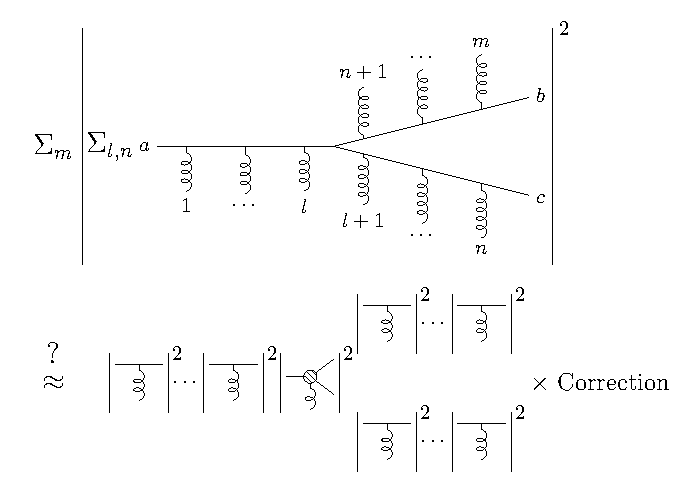
\includegraphics[width=.8\textwidth]{splitting-approx.pdf}
\caption[A schematic demonstration of the ``modified transport'' approach.]{A schematic demonstration of the ``modified transport'' approach. We seek for an approximation to the coherent process by an incoherent transport simulation with a multiplicative correction to the branching probability.}
\label{fig:split-approx}
\end{figure}
\subsection{Modifying single particle evolution}
To see how to approximate the branching using a modification to the Boltzmann equation, we first go back to the branching probability formula introduced previously \cite{CaronHuot:2010bp},
\begin{eqnarray}
\frac{dP^{a}_{bc}}{dx} &=& \int_0^\infty dt \frac{g^2 P(x)}{2\pi x (1-x) } \int_t^\infty dt'  F(t', t).
\label{eq:full-theory}
\end{eqnarray}
We have abbreviated the transition amplitude by the notation $F(t', t)$ for convenience, but always keep in mind this is a quantity that depends on $E, \omega, g$ and complete medium properties along the trajectory of the parton, including temperature and fluid velocity profiles $T(t), u^\mu(t)$.
The obstacle towards the Boltzmann formulation is the double-time integral that is the signature of the quantum transition, which also suggests a fundamental change to the semi-classical approach.

If the time-dependent wave-function is expanded in a series of the collision operator, then this transition amplitude includes the superposition of an arbitrary number of multiple-interaction with the medium.
Though multiple collisions of the branching partons are also present in the Boltzmann simulation, the difference is that the Boltzmann multiple collisions are independent of the branching processes; therefore, they only broaden the relative transverse momentum {\it without} changing the branching probability.
From the leading-log approximation, we see that the branching probability should be reduced by a factor $\sim \lambda/\tau_f$.
Our modified approach follows this simple observation, and can be summarized as follows (please also refers to figure \ref{fig:split-approx} for a schematic demonstration).
\begin{itemize}
\item[1.] Assume an incoherent branching process is generated at $t=t_0$. Do not treat the daughter partons as immediately independent.
\item[2.] Both mother and daughter partons receive elastic broadening from interacting with the medium, which also changes the formation time of the branching.
\item[3.] Evolve the branching system until $t-t_0 > \tau_f$. Then, reject this branching process with an acceptance probability that is proportional to $\lambda/\tau_f$, which corrects for the fact that these multiple scatterings should contribute coherently.
\item[4.] Branching partons for those accepted processes are treated as independent objects from this point; rejected partons are discarded without causing any physical effect.
\end{itemize}

Now we shall explain this scheme in detail.
Formally, this method can be understood as replacing the $F(t',t)$ by an ensemble average over $N$ copies of the branching systems using the following ansatz,
\begin{eqnarray}
F(t', t) \rightarrow \frac{1}{N}\sum_{i=1}^N \frac{b}{\tau_i(t)} \delta(t-t'- a \tau_i(t)).
\end{eqnarray}
Each copy ``$i$'' evolves independently and its formation time can be computed at any given time from the momentum space information,
\begin{eqnarray}
\tau_f(t) = \frac{2x(1-x) E}{k_\perp^2(t)}.
\end{eqnarray}
It is a function of time because elastic interactions changes the transverse momentum over time.
The $\delta$-function requires that a parton branching that starts at time $t'$  only forms at a latter time $t+a\tau_f$.
The inverse time scale $b/\tau_f$ contains the scaling of the rate: a certain amount of radiation is induced every formation time.
Such a particle-based representation of the two-point function $F(t', t)$, is indeed a crude ansatz, and its validity has to be tested later.
The dimensional numbers $a$ and $b$ shall be determined later when matching the prediction of this ansatz to the leading-log and next-to-leading-log calculations introduced in the previous section.

Plug this ansatz for $F(t, t')$ into the branching probability,
\begin{eqnarray}
\frac{dP^{a}_{bc}}{dx} &=& \frac{1}{N}\sum_i \int_0^\infty dt \frac{g^2 P(x)}{2\pi x (1-x)} \frac{b}{\tau_i} \\  
 &=& \frac{1}{N}\sum_i \int_0^\infty dt \frac{g^2 P(x)}{2\pi x (1-x) \tilde{\lambda}} \frac{b \tilde{\lambda}}{\tau_i(t=t'+\tau_i)}.\\
  &=& \frac{1}{N}\sum_i \int_0^\infty dt \frac{dR_{\textrm{incoh}}}{dx} \frac{b \tilde{\lambda}}{\tau_i(t=t'+\tau_i)}.
\end{eqnarray}
In the second line, we divided and multiplied back an effective mean-free-path $\tilde{\lambda} = m_D^2/\hat{q}_g$.
In doing so, the first factor is interpreted as the incoherent branching rate $R_{\textrm{incoh}}$, while the second factor is simply the acceptance factor for incoherent branching samples we introduced before.
The formation time can be determined self-consistently for each branching copy as it is evolved under the influence of elastic broadening.
It is determined at the time when
\begin{eqnarray}
t - t' < \tau_f(t). 
\end{eqnarray}
This iterative approach for determine $\tau_f$ was first developed and implemented by \cite{Zapp:2011ya}.
In the deep-LPM region where the number of rescattering is large, such a procedure reproduces the expected scaling of the average formation time $\left\langle\tau_f\right\rangle \propto \sqrt{\omega/\hat{q}}$.
This approach also generalizes to a medium with a varying temperature profile because the multiple collisions are performed along the trajectory of the probe.
In cases where the formation time is short so that the acceptance probability is bigger than unity, the acceptance is set to one and the incoherent rate recovers the Bethe-Heitler results.
Therefore, this approach naturally provides an interpolation of the deep-LPM regime for energetic branchings and the Bethe-Heitler regime for soft branching in a large medium.

\paragraph{Determination of the $a$ parameter} Now we will determine the form of parameters $a$ and $b$ with guidance from the theory in the deep-LPM region.
In the leading-log formula, the average inverse formation time is $\langle\tau_f^{-1}\rangle \sim \sqrt{\hat{q}_3 / 2x(1-x)E}$. 
One notice that the effective $\hat{q}_3$ is different from the $\hat{q}$ of the daughter parton 
$\hat{q}_3$ is related to the gluon $\hat{q}$ by the process- and $x$-dependent factor $C_{abc}$ that has been defined before.
For this reason, we chose the $a$ parameter to be the color combination for each branching channel.
\begin{eqnarray}
a \rightarrow a_{abc}(x) = \frac{C_b}{C_{abc}(x)}
\end{eqnarray}

\paragraph{Determination of the $b$ parameter} From the previous theory discussion, we know that there is a logarithmic ambiguity in the cut-off scale $Q_0$ in $\hat{q}_3$, which can be determined at the NLL level to be the same order as the branching transverse momentum.
We need to address what the $Q_0$ scale is in the Boltzmann simulation and how to improve on that.
Because the large-$Q$ part of the elastic rescattering also uses vacuum two-body matrix-elements, the upper bound of the momentum transfer integration is cut-off by the center-of-mass energy $\sqrt{s}$ of each independent collision,
\begin{eqnarray}
s = (p_1 + p_2)^2 = 2E_1 E_2 (1-\cos(\theta))
\end{eqnarray}
where $p_1$ and $p_2$ are the four momenta of the hard parton and the medium parton.
Since at high energy, the cross-section evolves slowly with $\sqrt{s}$, we can define the average $\sqrt{s}$ by simply averaging $p_2$ over the thermal distribution,
\begin{eqnarray}
2p_1\frac{ \int p_2^3 e^{-p_2/T}(1-\cos\theta) dp_2 d\cos \theta }{\int p_2^2 e^{-p_2/T} dp_2 d\cos \theta} =  6ET.
\end{eqnarray}
Therefore, the average $Q_0^2$ from the independent transport simulation is $6ET$, compared to the NLL choice of $\sqrt{\hat{q} \omega}$
The predictions from such a simulation would systematically deviate from theory predictions in a logarithmic manner, varying energy, temperature and coupling constant.
To use the correct scale, we define a scale-dependent acceptance probability to correct the na\"ive choice of $Q_0 \sim \sqrt{6ET}$ with a $b$ parameter,
\begin{eqnarray}
b &=& 0.75\sqrt{\frac{\ln(\hat{Q}_1^2 )}{\ln(\hat{Q}_0^2 )}}.
\label{eq:NLL-b}
\end{eqnarray}
with $\hat{Q}_1^2$ and $\hat{Q}_0^2$ given by,
\begin{eqnarray}
\hat{Q}_1^2 &=& 1 + \frac{\sqrt{2x(1-x)E\hat{q}}}{m_D^2} \approx 1 + \frac{\tau_f}{\tilde{\lambda}}\\
\hat{Q}_0^2 &=& 1 + \frac{6ET}{m_D^2}
\end{eqnarray}
The $0.75$ is a constant determined when the simulation is tuned to theoretical calculations in the next section, and it will be the same throughout the entire work.
This logarithmic ambiguity traces back to the cut-off $Q_0$ imposed on the large-$q^2$ perturbative tail of $\hat{t}$-channel matrix-element;
therefore, if one assumes the absence of such a tail\footnote{\singlespacing For example, non-perturbative physics motivated coupling between the hard parton and the medium}, one should drop this logarithmic part in the $b-$parameter.

\subsection{Implementing mass effect}
To apply the aforementioned approach to study heavy flavor, we require
the limit that the parton energy is large compared to the heavy quark mass.
Considering that heavy quarks introduce a mass correction to the Fermion propagator, a {\it na\"ive } change is to include the mass effect in both the formation time and also the few-body matrix-elements,
\begin{eqnarray}
\tau_f = \frac{2x(1-x)E}{k_\perp^2} \rightarrow \frac{2x(1-x)E}{k_\perp^2 + x^2 M^2}
\end{eqnarray}
and 
\begin{eqnarray}
\overline{|M|^2}_{2\leftrightarrow 2}(m=0) \rightarrow \overline{|M|^2}_{2\leftrightarrow 2}(m=M)\\
\overline{|M|^2}_{2\leftrightarrow 3}(m=0) \rightarrow \overline{|M|^2}_{2\leftrightarrow 3}(m=M)
\end{eqnarray}
For elastic scatterings, this replacement using the massive version of the two-body matrix-element is justified because subsequent elastic collisions are incoherent in the weak coupling limit.
For inelastic scatterings, again, the problem arises from the coherence over multiple scattering centers.
At high energy, a heavy quark acquires an average transverse momentum $\hat{q} \tau_f$ larger than the typical transverse momentum of the few body matrix-element $\overline{|M|^2}_{2\leftrightarrow 3}$.
As a result, the mass-effect should be less important compared to the scale $\hat{q} \tau_f$ than comparing to the transverse momentum acquired from a single collision center. 
To solve this problem in the simulation, we choose to use the dead-cone approximation for the radiation from a heavy quark.
The $2\rightarrow 3$ and $1\rightarrow 2$ branching of the heavy quark is sampled from the massless calculation, while the formation time is determined using the massive formula.
The key change is that the dead-cone factor modifies the acceptance probability,
\begin{eqnarray}
\frac{b\lambda}{\tau_f} \rightarrow \frac{b\lambda}{\tau_f} \left(\frac{k_\perp^2}{k_\perp^2+x^2M^2}\right)^2.
\end{eqnarray}
Note that the $k_\perp$ here is the branching transverse momentum after the elastic broadening, and on average $\langle k_\perp^2 \rangle = \langle k_{0,\perp}^2 \rangle + \langle\tau_f\hat{q}\rangle$, where $\langle k_{0,\perp}^2 \rangle$ is the average transverse momentum sampled from the $2\rightarrow 3$ matrix-element.
One may question the accuracy of approximating the massive version of the complicated multiple scattering matrix-element using a dead-cone approximation.
We will compare the radiation spectrum from the heavy quark to the exact solution for heavy quark in the next section.

\subsection{Implementing the running of $\alpha_s$}
There are two places in the transport model where the running of the strong coupling constant is relevant:
the coupling between the hard parton and the medium, and the coupling constant for the branching vertices.
These two processes often happen at different scales.

For elastic interactions, the scale would be the $\hat{t}$-channel momentum transfer, the typical scale is on the order of the screening mass $|\hat{t}| \sim m_D^2$.  
Using leading order running of $\alpha_s$ $n_f = 3$ and $\Lambda = 0.2$ GeV, 
\begin{eqnarray}
\alpha_s(Q^2) = \frac{4\pi}{9\ln\left(Q^2/\Lambda^2\right)}
\end{eqnarray}
the coupling constant will blow up with the scale getting close to the non-perturbative scale $\Lambda^2$, and applying a leading-order perturbative calculation to such regions is problematic. 
In a medium, we introduce a minimum scale in the running coupling, proportional to the temperature $Q_{\textrm{med}} = \mu \pi T$, to regulate the leading order running formula.
Of course, regulating $\alpha_s$ to a finite value using such a medium scale does not necessarily improve the accuracy of the calculation in this temperature range. 
For example, $\alpha_s(2\pi T)$ ranges from $0.28$ to $0.45$ ($g \sim 1.9$--$2.4$) for temperature decreasing from $T=0.4$ GeV to $T_c$, which are extremely large values, considering that the next-to-leading-order correction to the probe-medium correction is $O(g)$  
\footnote{\singlespacing As a remark, in the final model-to-data comparison, we try to parametrize the non-perturbative contribution by a diffusion processes in our model to prevent the attempt to explain the coupling to sQGP in a pure perturbative framework.}.
Following \cite{Arnold:2008zu}, the elastic collision couplings are evaluated at the $\hat{t}$-channel momentum transfer $q_\perp^2$.
This involve both the $\alpha_s$ in the large-$q$ matrix-element ($2\leftrightarrow 2$, and the elastic matrix-element factorized in $2\leftrightarrow 3$) as well as the $\alpha_s$ in the soft transport coefficients $\hat{q}_S$ and $\hat{q}_{L, S}$.

Unlike the coupling between hard parton and the medium, the scale for the splitting process is much harder than the screening mass due to transverse momentum broadening. For example, in a static medium,  $k_\perp^2$ scales like $\sqrt{2x(1-x)E\hat{q}} \sim m_D^2 \sqrt{\omega/T}$.
Therefore for splitting where both the daughter patrons are hard $xE, (1-x)E \gg T$, the running of the splitting vertex coupling is under better control than the probe-medium coupling.
The running of the splitting vertex is included in the theory by changing the $\hat{q}_3$ in the NLL formula to its running version  \cite{Arnold:2008zu},
\begin{eqnarray}
\hat{q}_3^{\textrm{running}} \approx \frac{4\pi}{9}\left(g^2(m_D^2) - g^2(Q_0^2)\right) 1.27 T^3 C_{abc}(x),
\label{eq:q3running}
\end{eqnarray}
and then evaluate the splitting $\alpha_s$ around an averaged scale (note that $k_\perp^2$ in the simulation fluctuates a lot),
\begin{eqnarray}
\langle k_\perp^2\rangle \sim m_D^2 \sqrt{E/T\ln(E/T)}
\label{eq:runscale}
\end{eqnarray}  
For transport simulations, the running of splitting vertex requires a two-step implementation. 
First, the $\alpha_s$ for the splitting vertex in the few body matrix-element is evaluated at $k_\perp^2$.
Next, at the end of the elastic broadening for each splitting processes, the acceptance probability is multiplied by a running coupling factor
\begin{eqnarray}
p_{\textrm{running}} = p\times \frac{\alpha_s(k_{\perp,t_0+\tau_f}^2)}{\alpha_s(k_{\perp,t_0}^2)}.
\end{eqnarray}
Where $k_{\perp,t_0}^2$ is the transverse momentum when the splitting is generated from the few-body processes, while $k_{\perp,t_0+\tau_f}^2$ is the final transverse momentum including the elastic broadening, and is on average greater than $k_{\perp,t_0}^2$.

\section{Validating the modified transport approach}
\label{section:valiate_lido}
In this section, we compare the simulation of the ``modified Boltzmann transport'' to theoretical calculations introduced in the previous sections for different parton energy, coupling constants, and medium temperatures that are relevant for phenomenological applications.
Such a model validation is crucial as it tells us whether the model is a good proxy of the underlying theory and quantifies the theoretical uncertainty when applying the model to phenomenological studies and transport parameter extraction.

We first compare the splitting rate $dR/d\omega$ that comes out of the modified Boltzmann simulation to the NLL approximation in the infinite medium limit.
Then, we apply the model to a finite and expanding medium, outside of the region where this approach is designed.
Nevertheless, the model achieves a good qualitative agreement with the theoretical calculation of the finite size effect
In the end, we validate the implementation of the heavy quark mass effect.

\subsection{In a large and static medium}
\begin{figure}
\singlespacing
\centering{
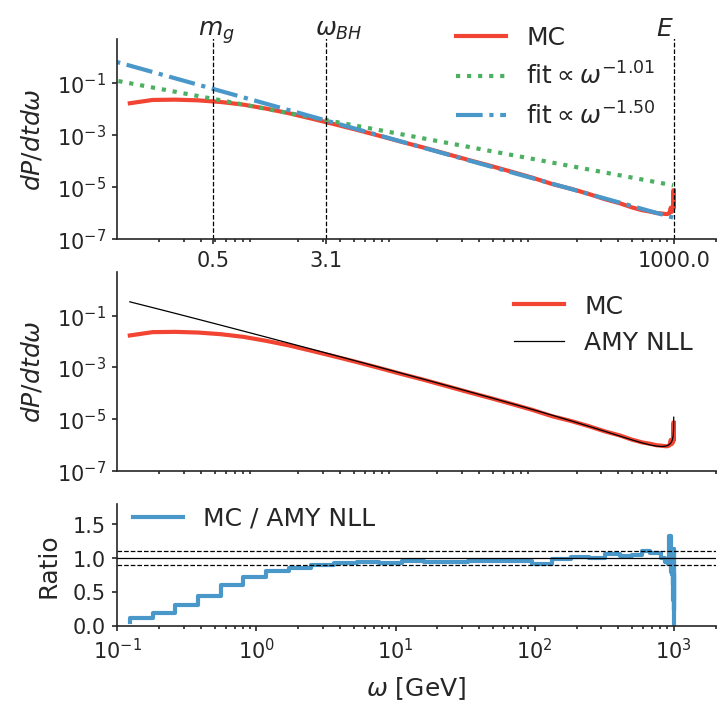
\includegraphics[width=.8\columnwidth]{spectrum.png}
}
\caption[The $q\rightarrow q+g$ splitting rate simulated in an infinite box with]{The $q\rightarrow q+g$ splitting rate simulated in an infinite box with $T=0.5$ GeV. The quark energy is $E=1$ TeV. $\alpha_s = 0.1$. In the top plot, the spectrum $dR/d\omega$ (red line) is fitted to a power function $\omega^\lambda$ in different gluon energy regions. The green dashed line is fitted in the Bethe-Heitler region $\omega < \omega_{BH}\approx 2\pi T$; the blue dash-dotted line is fitted in the LPM region $\omega > \omega_{BH}$. The middle plot compares to the simulation to NLL solution to the AMY equation, and their ratio is shown in the bottom plot.}
\label{fig:spectrum}
\end{figure}

In practice, to define a Monte-Carlo transport simulation in an infinite medium limit and an eikonal limit of parton propagation, an ensemble of partons of a certain species is initialized at a fixed energy $E_0$ and will be let to propagate in the ``$+z$'' direction.
Each time when a parton scatters elastically or splits, its splitting kinematics ($\omega, k_\perp, t_0, \tau_f$) is recorded, then the mother parton's energy is reset back to its initial value (a test in the eikonal limit).
For elastic re-scatterings in the implementation of the LPM effect, the parton's energy is re-scaled back to the value before scatterings without changing its direction.
The system is evolved for a sufficiently long time $t_{\max}$, and only branchings that takes place within $[t_{\min}, t_{\max}]$ are analyzed to focus on the infinite time behavior of the simulation.

We start with the result for $q\rightarrow q+g$ channel shown in 
figure \ref{fig:spectrum}.
It displays the differential rate $dR/d\omega$ for a 1 TeV quark propagating through a medium of $T=0.5 GeV$ with coupling constant $\alpha_s = 0.1$.
The switching scale parameter takes a default value $Q_{\textrm{cut}}^2 = 4 m_D^2$
The vertical axis is the differential branching rate $dR/d\omega$, and the horizontal axis is the energy of the final state gluon $\omega$.
To better understand our result, we have put three ``landmark'' energy scales in the upper plot, which are the initial parton energy $E$, an estimate of the Bethe-Heitler energy $\omega_{\textrm{BH}}\sim\hat{q}_g \lambda_g^2 \sim 2\pi T$, and the screening mass $m_g = m_D/\sqrt{2}$.
In the LPM regime $\omega_{\textrm{BH}} < \omega$, the spectrum falls off as a power law with fitted exponent $-1.50$ (the blue dash-dotted line), and in the Bethe-Heitler regime above the screening mass $m_g < \omega < \omega_{\textrm{BH}}$, the fitted power law exponent is close to $-1$ (the green dotted line).
These exponents are in good agreement with the theoretical expectation that $dR_{\textrm{BH}}/d\omega \propto \omega^{-1}$ and $dR_{\textrm{LPM}}/d\omega \propto \omega^{-3/2}$ from equations \ref{eq:incoh-dR} and \ref{eq:AMY-LL}.
The screening mass regulates the soft divergence of the spectrum below $m_g$.
One may notice a tiny increase of the spectrum when $\omega \rightarrow E$, this is a region where the gluon takes a larger fraction of the initial quark's energy.

In the middle plot, we compare the NLL solution directly to the simulated results.
As a remark, we have tuned the prefactor in the $b$-parameter to be $0.75$  by comparing to this theory prediction at $\alpha_s=0.1, E=1 \textrm{TeV}, T = 0.5 \textrm{GeV}$ for the $q\rightarrow q+g$ channel.
For the rest of the comparison with different coupling, parton energy, temperature, and channels, this parameter will {\bf not} be further tuned.
The simulation agrees with the NLL solution very well when $\omega \gg \omega_{\textrm{BH}}$ where the formula is valid.
The bottom plot shows the ratio between the simulation and the theory, and it achieves a level of $\pm 10\%$ agreement in the deep-LPM region.

\begin{figure}
\singlespacing
\centering{
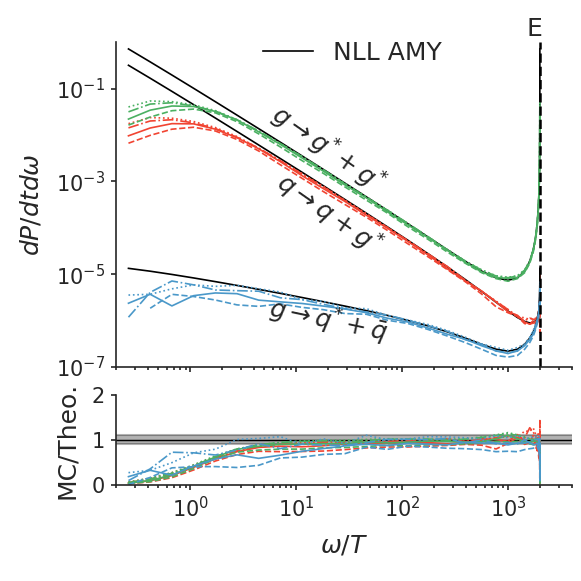
\includegraphics[width=.8\columnwidth]{channel_rate.png}
}
\caption[Top plot shows the rates of different channels $q\rightarrow q+g^*$,]{Top plot shows the rates of different channels $q\rightarrow q+g^*$, $g\rightarrow g+g^*$, and $g\rightarrow q^* + \bar{q}$ are plotted as functions of the daughter (labeled by ``${}^*$'') parton energy. The mother parton has a energy $E=1$ TeV. The medium temperature is $T=0.5$ GeV. $\alpha_s = 0.1$. The simulations (colored lines) are compared to the NLL solutions (black lines). Different line shapes use $Q_{\textrm{cut}}^2 = 2m_D^2$ (dashed), $4m_D^2$ (solid), $8m_D^2$ (dash-dotted), and $16 m_D^2$ (dotted).
The ratios between the simulated results and theory are shown in the bottom plot.}
\label{fig:channel_rate}
\end{figure}

Next, we compare the simulation with all the three channels in figure \ref{fig:channel_rate}.
The setup is the same as the figure \ref{fig:spectrum}.
The red, green and blue lines correspond to the differential branching rate of processes $q\rightarrow q+g^*$, $g\rightarrow g^*+g^*$ and $g\rightarrow q^*+\bar{q}$; the thin back lines are the NLL solution to the AMY equation.
The ``${}^*$'' sign denotes the final-state partons whose energy  $\omega$ are recorded.
For the case of two final state gluons, both are taken into account in the simulation as they are identical particles.
We have discussed the feature for the $q\rightarrow q+g$ process in the previous paragraph. 
The spectral shape of the $g\rightarrow g+g$ process is very similar to the quark splitting channel in the range $\omega \ll E$, with a higher value.
The rate is symmetric with respect to $\omega = E/2$ due to its symmetric final states (though it is hard to tell from this double-log plot), so at large $\omega$, the rate goes up again.
The spectrum of $g\rightarrow q+\bar{q}$ is also symmetric with respect to $\omega = E/2$. Though its final state consists of two different particles,  the splitting function is symmetric.
We see that the simulation achieves a good agreement with the NLL solution in the deep-LPM region $\omega/T > 10$.
Furthermore, in this plot, we vary the switching scale $Q_{\textrm{cut}}$ between the diffusive coupling and scattering-like coupling between the probes and the medium.
The choices are $Q_{\textrm{cut}}^2 = 2 m_D^2$ (dashed lines), $4 m_D^2$ (solid lines), $8 m_D^2$ (dash-dotted lines), and $16 m_D^2$ (dotted lines).
First, the results do depend $Q_{\textrm{cut}}$.
Second, varying $Q_{\textrm{cut}}$ by a factor of $8$ only results in a $\sim 10 \%$ change in the magnitude of the spectra.
In particular, the strongest $Q_{\textrm{cut}}$ dependence appears when using the two smallest choices of  $Q_{\textrm{cut}}^2 = 2 m_D^2$ and $4 m_D^2$.
Once the switching scale is well above the Debye mass, the $Q_{\textrm{cut}}$-dependence is even weaker.

\begin{figure}
\singlespacing
\centering
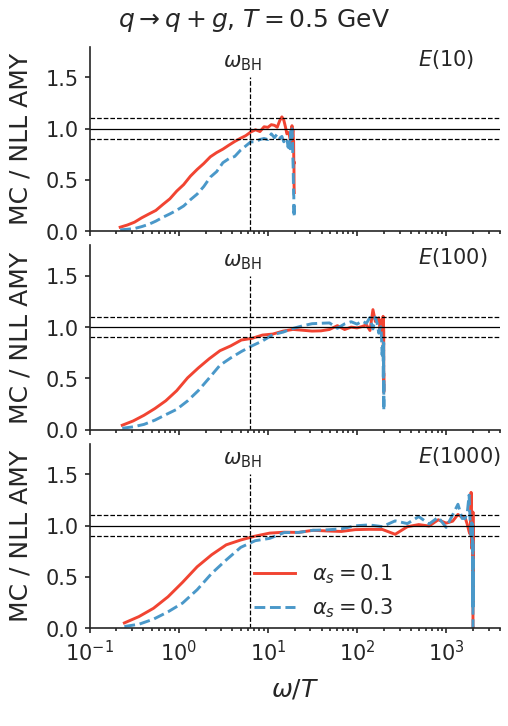
\includegraphics[width=.8\columnwidth]{spectrum_E_q2qg.png}
\caption[Ratios of splitting rate $dR/\omega$ between the modified Boltzmann]{Ratios of splitting rate $dR/\omega$ between the modified Boltzmann simulation and the NLL solution for $q\rightarrow q+g$ splitting. The quark energies are $E = 10$, 100, and 100 GeV from top to the bottom plot. 
And two coupling constants are used: $\alpha_s = 0.1$ (red solid lines) and $\alpha_s = 0.3$ (blue dashed lines).
$\omega$ stands for the gluon energy.
The horizontal dashed lines denote $\pm 10\%$ deviation from unity.}
\label{fig:sys-q2qg}
\end{figure}

Next, we test the model using different values of the coupling constant and parton energies.
We choose both a relative small coupling $\alpha_s = 0.1~(g \approx 1.12)$ and a value closer to the phenomenology coupling $\alpha_s = 0.3~(g \approx 1.94)$, and vary the energy from $10$, $10^2$, to $10^3$ GeV.
The ratios between the simulation and the NLL solutions are shown in figure \ref{fig:sys-q2qg}, \ref{fig:sys-g2gg} and \ref{fig:sys-g2qqbar}.
From these systematic comparisons,
one sees that the simulation reproduces the correct scaling in the LPM region, although this region shrinks due to the decrease of the parton energy.
In conclusion, the overall performance of the modified Boltzmann transport in describing the inelastic processes in a large medium is good and under control.
One remaining problem is that the systematic deviation for the $g\rightarrow q+\bar{q}$ channel is bigger than the other two channels, and we discuss on the cause of this in appendix \ref{app:ME}.

\begin{figure}
\singlespacing
\centering
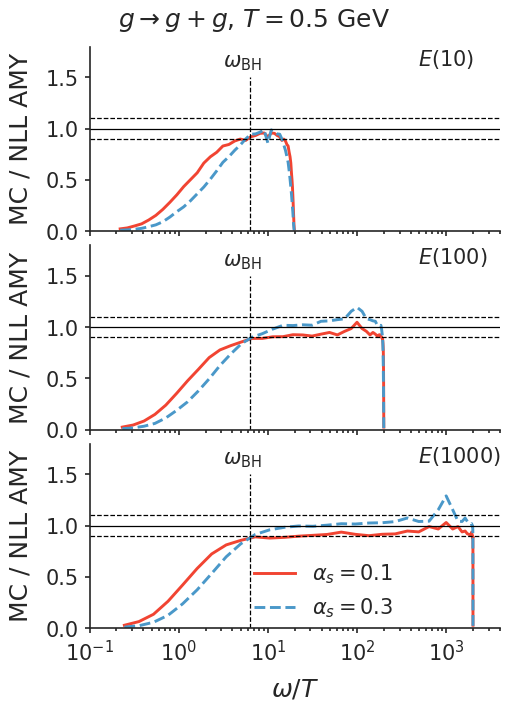
\includegraphics[width=.8\columnwidth]{spectrum_E_g2gg.png}
\caption{The same as figure \ref{fig:sys-q2qg}, but $g \rightarrow g + g$.}
\label{fig:sys-g2gg}
\end{figure}

\begin{figure}
\singlespacing
\centering
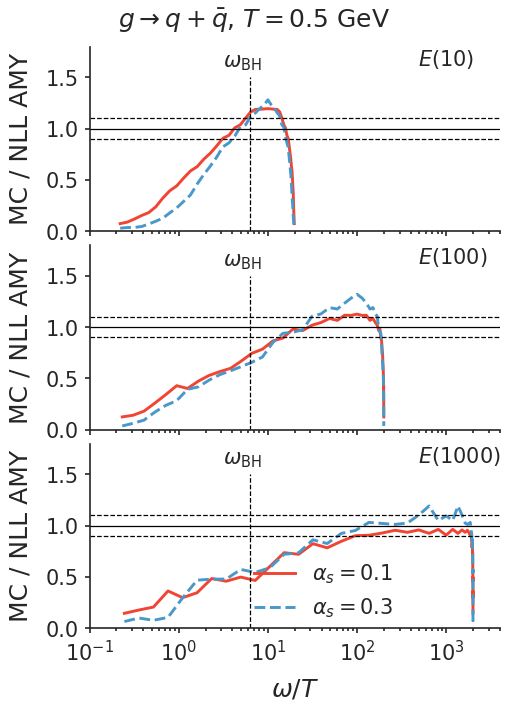
\includegraphics[width=.8\columnwidth]{spectrum_E_g2qqbar.png}
\caption{The same as figure \ref{fig:sys-q2qg}, but $g \rightarrow q + \bar{q}$.}
\label{fig:sys-g2qqbar}
\end{figure}

Finally, we validate the running coupling calculation in Fig. \ref{fig:running} using the $g\rightarrow g+g$ channel.
The theory curves (black lines) are obtained combining Eq. \ref{eq:AMY-LL} and Eq. \ref{eq:q3running}.
Different line styles correspond to the variation of the $Q_0$ value around an initial guess $m_D (E/T \ln(E/T) )^{1/4}$ by a factor of $2$ above and below.
For this 1 TeV parton, the scale $Q_0$ is large and the running of $\alpha_s$ is rather slow, which explains why the theory curve is not very sensitive to a factor of $4$ change in $Q_0$.
The simulation was performed using the running coupling prescription described in section \ref{section:modified-transport}.
The modified Boltzmann simulation again well describes the overall shape of the spectrum in the deep LPM region. 

\begin{figure}
\singlespacing
\centering
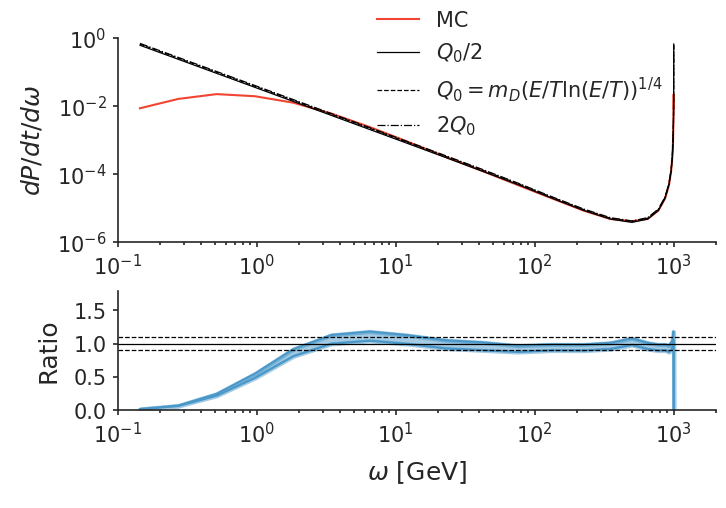
\includegraphics[width=.8\columnwidth]{running.png}
\caption[Comparing the simulation with running coupling constant to]{Comparing the simulation with running coupling constant to the NLL solution with running $\alpha_s$ prescription.
The scale $Q$ in the theoretical formula for the effective transport parameter $\hat{q}_3$ (equation \ref{eq:q3running}) is chosen to be $1/2$, $1$ and $2$ times of $\sqrt{\langle k_\perp^2\rangle}$ in equation \ref{eq:runscale}.
The ratio is shown in the bottom plot.}
\label{fig:running}
\end{figure}

\subsection{Branching in a finite / expanding medium}
We have made clear before that this approach is designed for interpolating between the Bethe-Heitler region and the deep-LPM region in a large medium, and looking at validation in the previous section; it indeed works very well.
However, the medium created in heavy-ion collisions is never in the large and static limit, its finite lifetime and spatial extension, local hot spot fluctuations and the fast radial expansion can all have a significant impact on the hard parton propagation. 
Therefore, we need to investigate how our approach would behave in a few more complicated cases including a finite medium and an expanding medium, before applying the model to phenomenological scenarios.

\paragraph{A semi-infinite medium}
Consider a semi-infinite medium with a static temperature profile,
\begin{eqnarray}
T = \begin{cases}
0 , z<0\\
T_0, z>0
\end{cases}
\end{eqnarray}
with hard partons being created at $z=0$ and propagating into the medium.
Deep inside the medium, the medium induced radiation should be asymptotically close to the calculation in an infinite medium.
At the boundary, there is a complicated interference between medium scatterings centers and the hard production vertex.
For a thin medium where the path length is short compared to the formation time, these interference terms can be worked out in the ``opacity expansion'', or by analyzing the propagator $G$ with a semi-infinite temperature profile.
This boundary effect results in a path length dependence of the medium induced branching rate that starts from zero at $t=0$ and gradually approaches the asymptotic value in a large medium.
The parton energy loss at the boundary scales quadratically with the path lenght  $\Delta E \propto L^2$ near the boundary; while it transits to $\Delta E \propto L$ deep inside the medium.

Indeed, we design the modified Boltzmann approach for the case of a large medium, but it also displays a certain finite size effect. 
Remember that the branchings in the modified transport approach take a finite amount of time, and those branchings that become independent at time $t$ are initiated by a $2\rightarrow 3$ processes from a wide range of scattering centers in the past $t' = t - \tau_f$.
Therefore, if the medium is semi-infinite, and there were no scattering centers before $t' = t-\tau_f < 0$, then the medium-induced contribution to the branchings at time $t$ are suppressed.
This reduction gets weaker and weaker when the condition $t-\tau_f > 0$ can be satisfied by more and more induced branchings and eventually, when $t\gg \langle \tau_f\rangle$, this boundary effect dies off in the simulation. 
Of course, we cannot achieve full quantitative agreement with the theory at $L \lesssim \tau_f$ since the detailed few-collision interference pattern is not implemented.
We would like to investigate if our simulation of the boundary effect can qualitatively mimic the interference physics that happens near the boundary.

\begin{figure}
\singlespacing
\centering
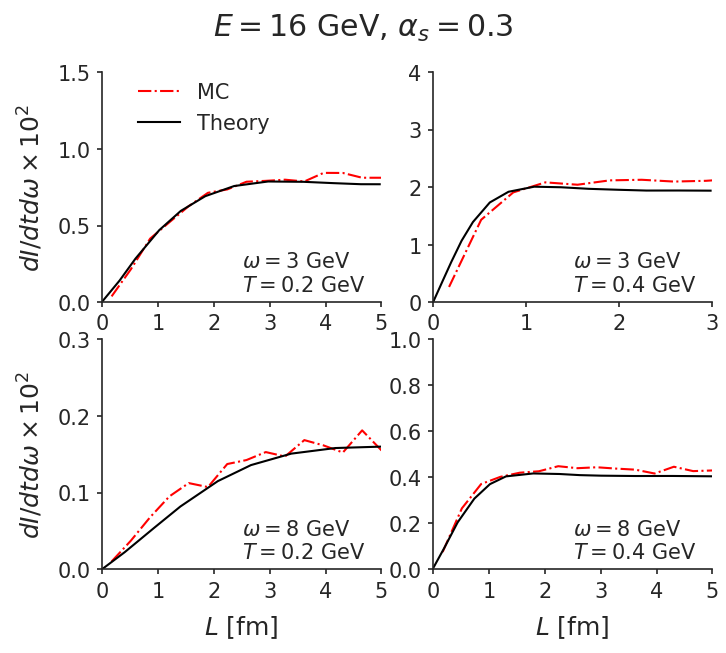
\includegraphics[width=.8\columnwidth]{spectrum_L.png}
\caption[The path-length dependence of the simulated $q\rightarrow q+g$]{The path-length dependence of the simulated $q\rightarrow q+g$ emission rate $dR/d\omega$ compared to the direction calculation of formula \ref{eq:full-theory} from \cite{CaronHuot:2010bp}. $\alpha_s = 0.3$. The quark energy is $16$ GeV. The left and right columns have medium temperature $T=0.2$ and $0.4$ GeV respectively. The top and bottom rows show the differential rate at $\omega = 3$ and $8$ GeV.}
\label{fig:spectra-L-alphas=0.3}
\end{figure}

In Figure \ref{fig:spectra-L-alphas=0.3}, the differential rate obtained from simulation is compared to the numerical solution of the full leading-order calculation for a finite medium.
The horizontal axis is the time of travel by the hard parton (path length divided by the speed of light), and each subplot shows how the branching rate changes as a function of time with different medium temperatures ($T=0.2$ GeV on the left, $T=0.5$ GeV on the right) and for different branching parton energy ($\omega=3$ GeV at the top, $\omega=8$ GeV at the bottom).
The theory curves are taken from reference \cite{CaronHuot:2010bp} for a 16 GeV parton with coupling constant $\alpha_s = 0.3$, and the red lines are our simulation.
The theory curve first increases linearly and then turn over to a constant value in the large medium limit for $t \gg \sqrt{2x(1-x)E/\hat{q}_3}$.
The simulation, as expected, reproduces the large time limit of the rate.
Moreover, we find that the current implementation also predicts the qualitative ``turn over'' of the spectra at finite path length.
The original paper only published this calculation for a $16$ GeV quark. 
To validate if this qualitative agreement also holds at higher parton energies, we implement the numerical approach of \cite{CaronHuot:2010bp} and compute the theoretical curves for $E=100$ GeV partons.
The comparison between simulation and numerical solutions are shown in figure \ref{fig:spectra-L-alphas=0.3-E100} and again, we find qualitative agreement with the theoretical finite size effect.

\begin{figure}
\singlespacing
\centering
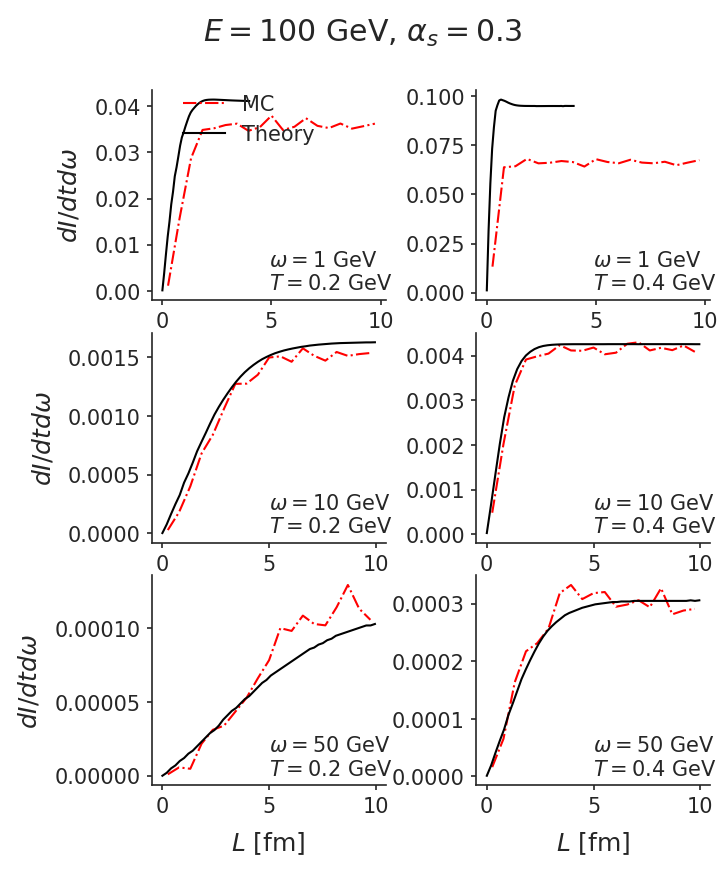
\includegraphics[width=.8\columnwidth]{spectrum_L_100.png}
\caption[The same as figure \ref{fig:spectra-L-alphas=0.3-E100}, but the initial quark energy is $100$ GeV,]{The same as figure \ref{fig:spectra-L-alphas=0.3-E100}, but the initial quark energy is $100$ GeV, and is plotted for gluon at 5 (top), 10 (middle) and 50 (bottom) GeV.}
\label{fig:spectra-L-alphas=0.3-E100}
\end{figure}

\paragraph{An expanding medium}
Fast radial expansion is another important feature of the medium in heavy-ion collisions.
It causes the temperature to decrease drastically in the early stages of the expansion and introduces another time scale in which the medium temperature changes notably.
Assume a simplified power-law changing temperature profile
\begin{eqnarray}
T(\tau; \nu)^3 = T_0^3\left(\frac{\tau_0}{\tau}\right)^{2-1/\nu}.
\end{eqnarray}
The $\nu$ parameter controls the rate of expansion. 
$\nu = 1/2$ is the static medium limit, and $\nu=1$ is the Bjorken flow.
We can define the following medium expansion time, over which the transport parameter changes significantly,
\begin{eqnarray}
\tau_{\textrm{ex}} = \left(\frac{d\ln(T^3)}{d \tau} \right)^{-1} = \frac{\tau}{2-1/\nu}.
\end{eqnarray}
The larger the $\nu$ parameter is, the smaller the expansion time scale.
With $\tau_0 \sim 1$ fm/$c$, the expansion time scale can be short enough that energetic branchings already probe the changing temperature profiles within their formation time $\tau_f > \tau_{\textrm{ex}}$.
One consequence of this fast changing of temperature is that, for these branchings $\tau_f > \tau_{\textrm{ex}}$, the transition probability over a finite amount of time can not be well approximated by integrating rates that are calculated in an infinite box defined by the local temperature,
\begin{eqnarray}
\frac{dP(t_1, t_2)}{d\omega} \neq \int_{t_1}^{t_2} \frac{dR_{\infty}(T(t))}{d\omega} dt,
\end{eqnarray}
where the rate $R_\infty$ is obtained by solving the branching rate in the infinite medium setup. 
Transport models such as MARTINI and TEQUILA use this assumption \cite{Jeon:2003gi,Schenke:2009gb,Dai:2019hbi}.
Our approach takes the change of the medium temperature (and also flow velocity) into account.
It is possible as the rescattering procedure that determines amount of suppression is performed along the trajectory of the hard partons; therefore, naturally includes the effect of the cooling of the medium.
The expansion also changes the typical formation time determined by the rescattering procedure.
Recall that in a static medium the dimensionless combination that enters the leading-log formula is $t/\tau_f \sim t \sqrt{\omega/\hat{q}}$, but with a $\hat{q}$ that is decreasing with temperature.
The self-consistent determination of the formation time requires the following relation to hold on average,
\begin{eqnarray}
t_2 - t_1 &=& \frac{2x(1-x)E}{k_{\perp}^2(t_1) + \int_{t_0}^{t} \hat{q}(\tau) d\tau},\\
\hat{q}(\tau) &=& \hat{q}(\tau_0) \left(\frac{\tau_0}{\tau}\right)^{2-1/\nu}
\end{eqnarray}

\begin{figure}
\singlespacing
\centering
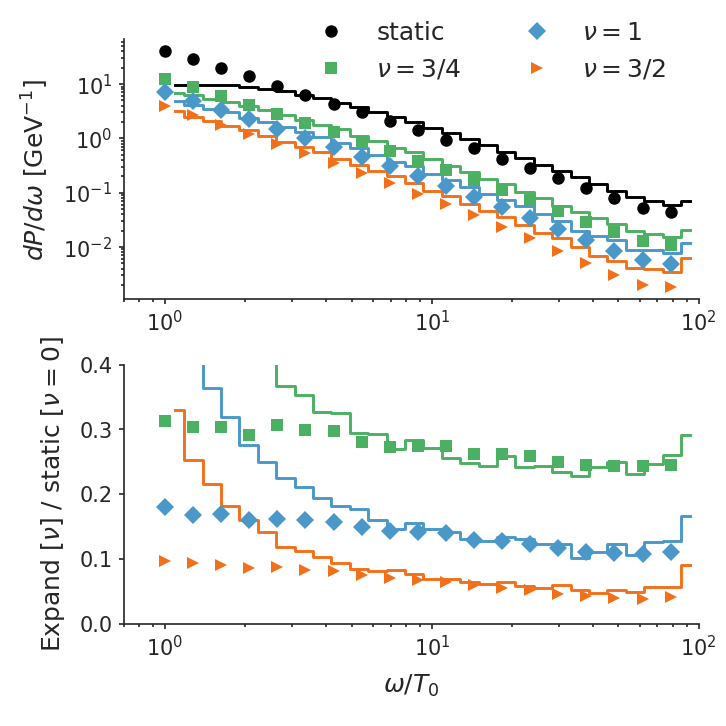
\includegraphics[width=.8\columnwidth]{spectrum_Bjorken.png}
\caption[Top plot: the simulated spectrum (diffusion plus diffusion-induced]{Top plot: the simulated spectrum (diffusion plus diffusion-induced radiation only) using the parametric medium with expansion parameters $\nu = 0$ (static, black), $3/4$ (green), $1$ (Bjorken, blue), and $3/2$ (orange). The analytic results are shown in symbols and simulations in lines. $\alpha_s=0.3$. The expansion starts at $\tau_0 = 0.2$ fm/$c$ with an initial temperature $T_0 = 1$ GeV. Bottom plot: the ratios between calculation (simulation) in an expanding medium to that in the static medium.}
\label{fig:Bjorken-BDMPS}
\end{figure}

Comparing to theoretical calculations, we utilize a result obtained in the BDMPS framework \cite{Baier:1996kr,Baier:1998yf}.
Using the power-law decreasing temperature profile, the obtained branching probability for the $q\rightarrow q+g$ splitting is \cite{Baier:1998yf},
\begin{eqnarray}
\frac{dP}{d\omega} &=& \frac{\alpha_s}{2\pi E}P_{q\rightarrow qg}(x)\mathfrak{Re}\int_{\tau_0}^{\tau_0+L}\frac{dt_f}{t_f}\int_{\tau_0}^{t_f}\frac{dt_i}{t_i} \frac{1}{\nu^2}\\
\nonumber
&& \left.\left[ I_{\nu-1}(z_i)K_{\nu-1}(z_f)-I_{\nu-1}(z_f)K_{\nu-1}(z_i)\right]^{-2}\right|_{\omega=xE}^{\omega=\infty},\\
z_{i,f} &=& 2i\nu \sqrt{\frac{\hat{q}_g(1-x+C_F/C_A x^2)}{2(1-x)\omega}} \tau_0 \left( \frac{t_{i,f}}{\tau_0}\right) ^{1/2\nu}.
\end{eqnarray}
This result recovers the static BDMPS result \cite{Baier:1996kr} when $\nu=1/2$.
One potential problem of comparing the formula to our simulation is that this BDMPS calculation works in the multiple-soft limit (leading log).
Therefore, we use only the diffusion-induced radiation in the simulation and deactivate the large-$Q$ $2\rightarrow 3$ scattering part.
Also, as mentioned before, in the absence of the perturbative tail in the collision kernel, $b=0.75$ is used without the logarithmic correcting factor in equation \ref{eq:NLL-b}.
Besides, we will not focus too much on the direct comparison between the spectra (top of figure \ref{fig:Bjorken-BDMPS}), but on the ratio between the expanding calculation/simulation over the static calculation/simulation (bottom of figure \ref{fig:Bjorken-BDMPS}).
This ratio reflects the change of the shape of the spectra due to the dropping of the temperature.

The simulation uses a medium with initial temperature $T_0=1$ GeV at $\tau_0=0.2$ fm/$c$ and lasts until $\tau = 20$ fm/$c$ using four different expansion rates $\nu = 1/2, 3/4, 1, 3/2$.
These choices correspond to a static medium, a slowly expanding medium, Bjorken flow, and a faster-than-Bjorken expansion.
We find that when $\omega \gg T_0$, the degree of change in the radiation spectra is well reproduced by the modified transport simulations.

\subsection{Comparison with a simplified solution of the transport equation}
Given the model mimic the single-emission vertex reasonably well, we move the focus to the full distribution function $f(t, \mathbf{x}, \mathbf{p})$ of partons propagated by the transport equation. 
The behavior of the distribution function is far more complicated than the final-state distribution of a single-emission vertex because transport equation resums multiple emissions during the time evolution.
Surprisingly, an analytic solution exists for a simplified version of the transport equation \cite{Blaizot:2013hx,Blaizot:2015jea}, which captures essential features of transport equation in the deep-LPM region.
The simplifications and assumptions are:
\begin{itemize}
\item Focus only on the longitudinal momentum distribution function in the high energy limit $f(t, \mathbf{x}, \mathbf{p})\rightarrow f(t, p_z \approx E)$. 
\item The initial condition consists of a single gluon $f = \delta(E-E_0)$.
\item Neglect elastic energy loss and use fixed coupling constant.
\item The system is gluonic. And retain only the singular part in the gluon splitting function $P_{gg}^g(0) = C_A(1+z^4+(1-z)^4)z^{-1}(1-z)^{-1} \rightarrow C_A z^{-1}(1-z)^{-1}$.
\item Consider the deep-LPM region ($\tau_f \gg \lambda$) in a large medium ($L\gg \tau_f$).
\item Use a leading-log picture where $\hat{q}$ is independent of the parton energy and neglect the difference between $\hat{q}$ and $\hat{q}_3$.
\end{itemize}
\begin{figure}
\centering
\singlespacing
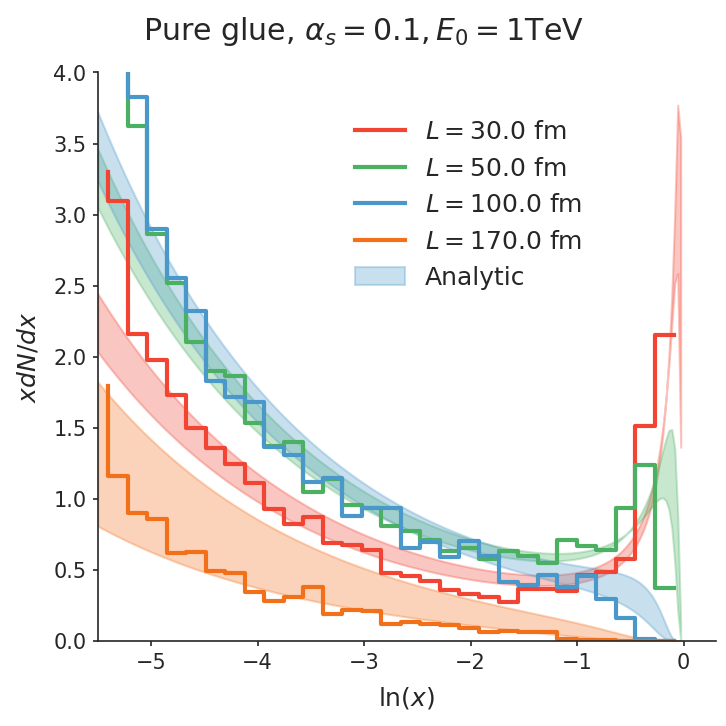
\includegraphics[width=.7\columnwidth]{jet_solution_NLL.png}
\caption[Comparing the simulated energy distribution shared among]{Comparing the simulated energy distribution shared among the hard partons to the simplified solution in equation \ref{eq:simple-jet-solution}. The value of effective $\hat{q}$ is varied from $\hat{q}_0\ln(2E\hat{q}_0/m_D^2)$ to $\hat{q}_0\ln(0.5 E\hat{q}_0/m_D^2)$ with $\hat{q}_0 = \alpha_s C_A T m_D^2$.}
\label{fig:jet_solution}
\end{figure}
Under these assumptions, the authors of \cite{Blaizot:2013hx} simplify the transport equation into, 
\begin{eqnarray}
\frac{\partial D(x, \tau)}{\partial \tau} = \int_x^1 \frac{dz}{z^{3/2}(1-z)^{3/2}} \sqrt{\frac{z}{x}} D\left(\frac{x}{z},\tau\right) -  \frac{D(x, \tau)}{\sqrt{x}}\int_0^1 \frac{z dz}{z^{3/2}(1-z)^{3/2}}.
\end{eqnarray}
$D(x, \tau) = E f(t, E=xE_0)$ is understood as the energy distribution with initial condition $D(x, \tau=0) = \delta(1-x)$.
$\tau = \alpha_s C_A/\pi \sqrt{\hat{q}/E_0} t$ is the rescaled dimensionless ``time'' variable. 
The gain-term and loss-term for the energy distribution are on the right-hand side.
The solution they obtained is 
\begin{eqnarray}
D(x, \tau) = \frac{\tau}{x^{1/2}(1-x)^{3/2}}e^{-\frac{\pi \tau^2}{1-x}},
\label{eq:simple-jet-solution}
\end{eqnarray}
which displays a simple $1/\sqrt{x}$ scaling at small $x$.
Indeed, this solution requires a series of approximations that is different from our modified transport models. 
For example, the rate in the model uses the full splitting function, and the elastic processes are intrinsic to the implementation of the LPM effect, and the elastic collisions cannot be turned off.
Moreover, the actual simulation always has a finite-size effect, which is not present in the simplified equation.
Nevertheless, qualitative features dominated by the singular part of the splitting kernel should be captured.

To see if the modified transport model reproduces such a feature, we initialize the system with an ensemble of $E_0=1$ TeV gluons in an infinite medium with temperature $0.5$ GeV.
The issue is the determination of $\hat{q}$ in the comparison because the effective $\hat{q}$ in the model is energy dependent $\hat{q} \sim  \hat{q}_0\ln(2x(1-x)E\hat{q}_0/m_D^2)$, with $\hat{q}_0 = \alpha_s C_A T m_D^2$.
We neglect the weak $x$-dependence and use two values $\hat{q}_0\ln(2E\hat{q}_0/m_D^2)$ and $\hat{q}_0\ln(0.5 E\hat{q}_0/m_D^2)$ in the theoretical formula.
In figure \ref{fig:jet_solution}, the simulated energy distribution (histograms) evolved to different path-length is compared to the simplified solutions using the two estimates $\hat{q}$ (colored bands).
The path-length where the finite-size effect is strong is $L_c = \sqrt{E_0/\hat{q}} \sim 15$ fm, so we have only compared the results for $L>L_c$.
We find a good agreement with the $1/\sqrt{x}$ scaling for large to model-small $x$ values, while the small-$x$ part of the simulation deviates from the expected trend.
One sees that the initial energy of the 1 TeV gluon at $x=1$ gets transported to the small-$x$ region; eventually, a significant fraction of energy is dissipated into the medium.

\section{Heavy quarks and thermalization test}
\begin{figure}
\singlespacing
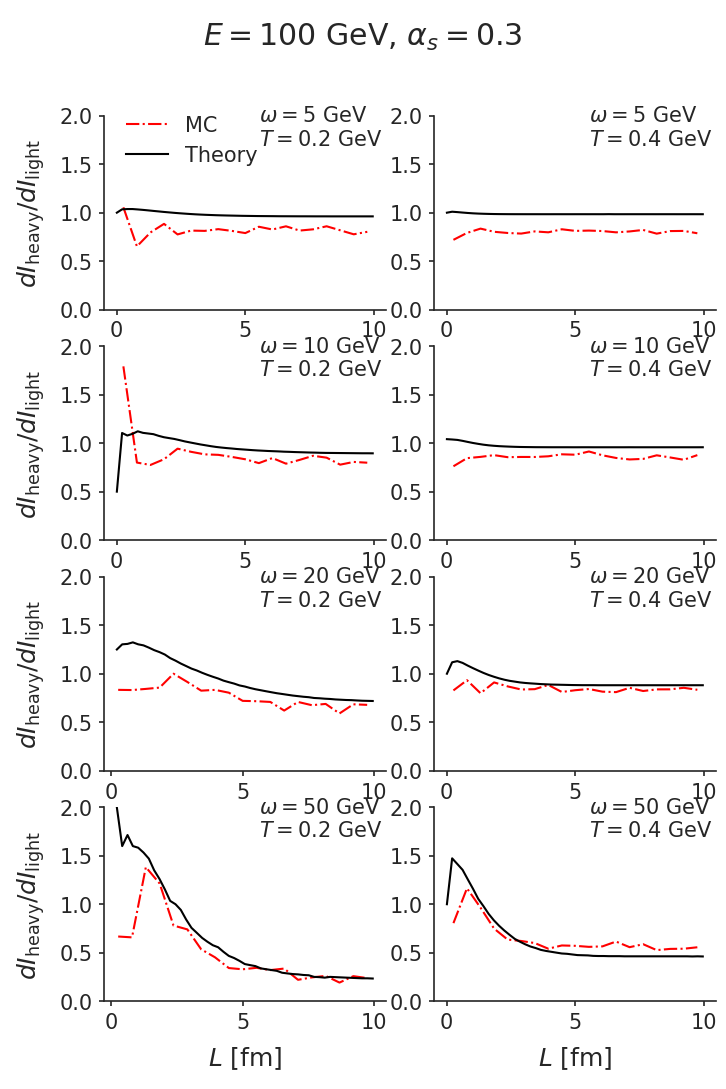
\includegraphics[width=\columnwidth]{mass.png}
\caption[The mass dependence of the radiation spectrum $q\rightarrow q+g$,]{The mass dependence of the radiation spectrum $q\rightarrow q+g$, presented as the ratio of bottom $dR/d\omega$ over the light quark $dR/d\omega$, as functions of path length. The left and right columns use temperatures 0.2 and 0.4 GeV. Different rows (from top to bottom) plot cases for gluon energy $\omega = 5, 10, 20, 50$ (GeV).}
\label{fig:mass}
\end{figure}
Finally, we check the model performance for heavy quarks.
The theory curves are obtained by solving the exact equation with an effective mass term,
\begin{eqnarray}
m_{\textrm{eff}}^2 = (1-x)m_g^2 + x^2 M^2
\end{eqnarray}
which includes both the thermal mass of the gluon and the current mass of the heavy quark.
We present the comparison between the simulation and the theory in terms of the ratio between the differential branching rate of the heavy quark (charm mass at 1.3 GeV, bottom mass at 4.2 GeV) and the light quark.
In figure \ref{fig:mass} for the bottom quark case, the horizontal axis is the path-length, and the vertical axis is the ratio.
Different rows have different radiated gluon energies, and different  columns have medium temperatures at $0.2$ GeV (left) and $0.4$ GeV (right) respectively.
The initial bottom quark energy is 100 GeV, and the coupling is $\alpha_s=0.3$.
We see that the dead-cone approximation agrees better with the theory calculation at larger $x$ and larger path-length.
Deviations observed at small path length are understood as the limitation of our implementation to the large medium and should be better treated by the opacity expansion. 
The deviation at small $x$ is interesting since the theory almost predicts an identical heavy quark radiation spectra as the light quark. 
This absence of a dead cone at small-$x$ is already observed in early works studying heavy quark energy loss in both the opacity expansion and the BDMPS framework \cite{Armesto:2003jh}.
It means that the treatment of the mass effect is not as simple as the dead-cone approximation and should be improved in the future.

\paragraph{Thermalization of heavy quarks}
\begin{figure}
\singlespacing
\centering
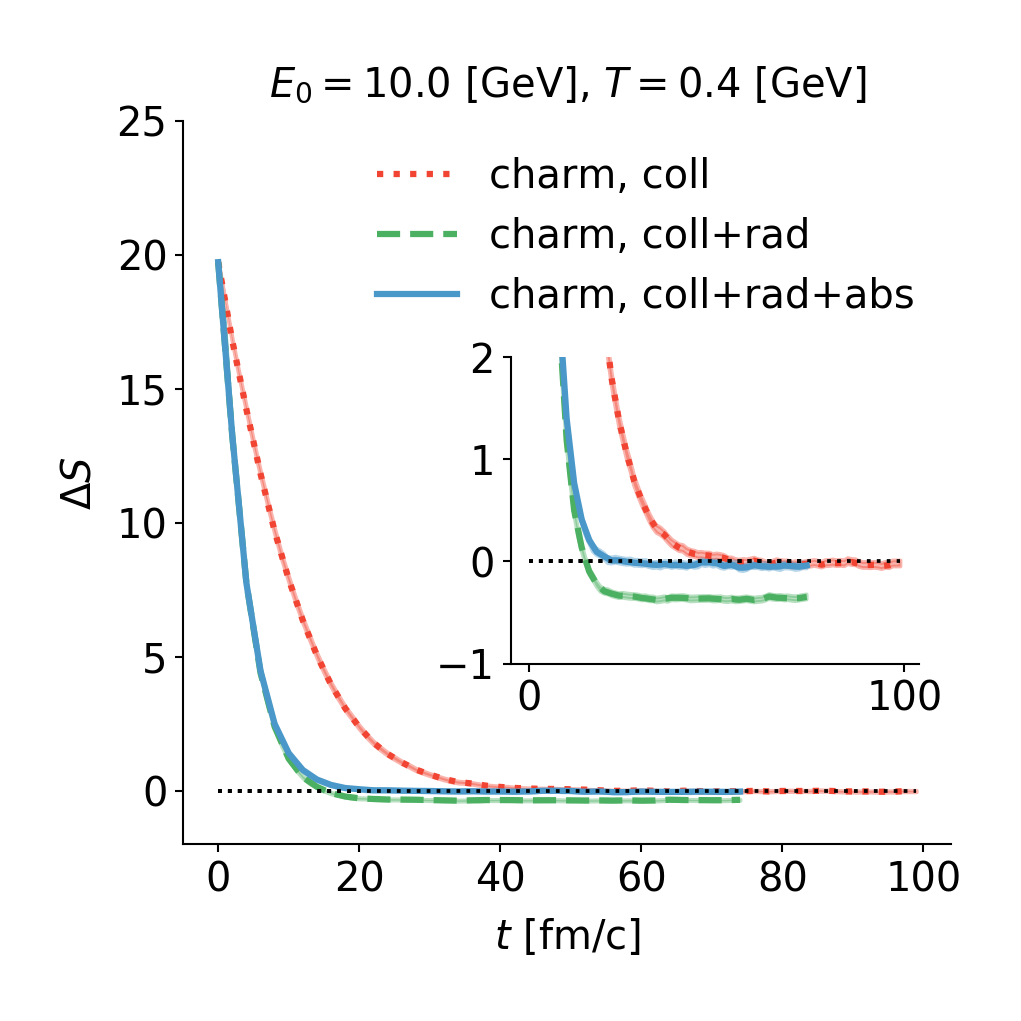
\includegraphics[width=.8\textwidth]{thermalization.png}
\caption[The approach to thermal equilibrium of heavy flavor is quantified]{The approach to thermal equilibrium of heavy flavor is quantified as the change of $\Delta S$ (defined in equation \ref{eq:DeltaS}) with time. The red dotted line includes elastic processes only. The green dashed lines= further includes $2\rightarrow 3$ and $1\rightarrow 2$ processes. The solid blue line turns on the detailed balance processes $3\rightarrow 2$ and $2\rightarrow 1$.}
\label{fig:thermalization}
\end{figure}
Due to a heavy quark's large mass, it takes a longer time to thermalize, and the low-$p_T$ end of the heavy quark production in the heavy-ion collisions can carry information on non-equilibrium dynamics.
To extract the degrees of thermalization, one has to make sure the correct thermal limit is achieved in the transport model, given sufficient time.
This is trivial for large-angle elastic scatterings and diffusion processes as long as the correct Einstein relation is imposed.
The $n\rightarrow n+1$ body radiative process is approximated by an initial $2\rightarrow 3$ or $1\rightarrow 2$ process and a sequence of elastic interactions; therefore, in principle, the $n+1\rightarrow n$ absorption processes need to be treated on the same footing to restore the detailed-balance in the modified-Boltzmann equation.
It can be done but is overly complicated.
Here we argue that close to a few times of temperature, the LPM effect is not that strong and an incoherent implementation of the absorption is enough to study the bulk of particles close to thermal distribution.

We define a quantity $\Delta S$ to measure the approach to thermal distribution $f_0 = e^{-E/T}$ for an ensemble of heavy quarks,
\begin{eqnarray}
\Delta S &=& - \langle \ln f_0 \rangle - S_0 \\
 &=& - \frac{1}{N}\sum_i\ln f_0(E_i) - \frac{\int dp^3 f_0 \ln(f_0)}{\int dp^3 f_0}
 \label{eq:DeltaS}
\end{eqnarray}
Where the first term is the ensemble average of the function $-\ln f_0$, and the subtracted term is proportional to the entropy of distribution $f_0$.
Note that the quantity is zero if the ensemble is thermalized.
If the system is approaching a thermal distribution with an effective temperature such that $f = e^{-E/T'}$, then $\Delta S$ is 
\begin{eqnarray}
\Delta S = \frac{\int dp^3 E/T e^{-E/T'}}{\int dp^3 e^{-E/T'}} - S_0 = \frac{T'-T}{T}
\end{eqnarray}
which is a measure of the deviation of the effective temperature from the thermal bath temperature.

Using this definition, we plot $\Delta S$ as a function of time for 1000 heavy quarks that are initialized at $E=10$ GeV.
The temperature of the thermal bath is 0.5 GeV, and we used a fixed $\alpha_s = 0.3$.
Under the influence of diffusion (red) and diffusion plus large-angle elastic collisions (green), $\Delta S$ decreases from a large value until fluctuating around zero after 25 fm/$c$ (red) and $15$ fm/$c$ (green).
Now, adding the radiative processes (blue), $\Delta S$ reaches a value below zero, which is a false equilibrium.
Only after the balancing processes of parton absorption are also included (orange), the correct thermal equilibrium limit restores. 
We also found that the absorption process only sets in when the ensemble is close enough to the thermal distribution, as the blue line and the orange line are almost overlapping until $\Delta S$ drops to 0.3.
This is because the absorbed gluon follows the thermal distribution in the medium while phase-space for a high energy parton $E\gg T$ to absorb a low energy gluon is very limited $x<T/E$, compared to radiation processes where the value of $x$ is not restricted by the Boltzmann factor $e^{-xE/T}$.

\section{Comments on two other inelastic process implementations}
\label{section:compare_former}
I find it beneficial to discuss two other inelastic process implementations for the reader's reference. 
They are termed as the ``coherence factor'' approach and the ``blocking radiation'' approach.
I have used the previous approach in my earlier studies \cite{Ke:2018tsh}, but it is the problems I encountered in this method that later motivated the development of the ``modified Boltzmann transport'' method. 
I shall show in this section that in the deep-LPM region, the ``coherence factor'' approach still qualitatively agrees with the power counting of the LPM suppression $\lambda_{el}/\tau_f$, though it only includes the effect of one medium scattering center and the method can be logarithmically dependent on the infrared cut-off.
The ``blocking radiation'' approach, however,  does not reproduce the correction magnitude of the LPM suppression.
These two approaches, together with the ``modified Boltzmann'' approach will be compared later using the ``energy loss'' of a fixed energy quark.

\subsection{The coherence factor approach}
This approach is first implemented in the improved Langevin equation \cite{Cao:2013ita}, using the single medium-induced radiation probability from the higher-twist calculation \cite{Majumder:2009ge,Wang:2001ifa} and a prescription for multiple emissions.
The higher-twist formula of medium-induced radiation is derived for a high virtuality parton, including the interference of the hard production vertex and one medium scattering center.
The single radiation rate reads,
\begin{eqnarray}
\frac{dN_g}{dx dk_\perp^2 dt} = \frac{\alpha_s P(x)\hat{q}_g}{\pi k_\perp^4} 2\left(1-\cos\frac{t-t_0}{\tau_f}\right), \tau_f = \frac{2x(1-x)E}{k_\perp^2}
\end{eqnarray}
Here the radiation rate is time-dependent ($t$) due to the interference with the hard production at time $t_i$. 
Note that the interference factor cancels the collinear divergence. 
The only divergence comes from soft emission $x\rightarrow 0$. 
This divergence is not a problem for computing more physical quantities such as energy loss, as gluon absorption processes will balance it.
However, an infrared cut-off $x>x_c$ has to be introduced to apply the rate equation formulation. 

The advantage is that if there is only one radiation, then the sampling of the time-dependent rate indeed reproduces the higher-twist calculation.
However, the ambiguity arises from the way it handles multiple emissions.
For example, one can compute the average number of emission by integrating this formula along the trajectory of the hard parton and then samples the fluctuating number of emissions with a Poisson distribution.
However, of course, this would assume the parton energy is not significantly changed during the process, and it is not clear how the presence of more than one scattering center would change this picture.
Here we would like to discuss another method in dealing with multiple emission using the higher-twist formula in a time evolution manner \cite{Cao:2013ita}.
The algorithm goes as follows:
\begin{itemize}
\item[1.] Choose an infrared cut-off for the gluon energy $x_c \propto T/E$, and a small enough time step $\Delta t$, so that the average number of emissions is much smaller than $1$ to suppress multiple emissions within $\Delta t$,
\begin{eqnarray}
\langle N_g \rangle = \Delta t \int_{x_c}^1 dx \int dk_\perp^2 \frac{dN_g(t-t_0)}{dx dk_\perp^2 dt} \ll 1.
\end{eqnarray}
\item[2.] Sample N according to a Poisson distribution with $\langle N_g \rangle$. For $\langle N_g \rangle \ll 1$, it is sufficient to sample the two leading cases of $N=0, 1$, as the probability to have more than 1 emission is negligible ($P_{N>2} = 1-e^{-\langle N_g \rangle}-e^{-\langle N_g \rangle}/\langle N_g \rangle = O(\langle N_g \rangle^2) \ll P_1 \ll P_0$).
\item[3.] If $N=0$ then propagate the parton to the $t+\Delta t$. If $N=1$, then sample the emission gluon's $x$, and $\vec{k_\perp}$ by the differential rate. {\it Meanwhile, $t_0$ is set to $t$}, so that the next emission's probability will be accumulated from zero again.
\item[4.] Proceed to the next time step.
\end{itemize}
We found that the key step here is resetting the clock $t_0 = t$ for the parton after every emission.
As a result, from the second emission onward, the $t-t_0$ that appears in the interference factor is measuring the time difference between two medium scattering centers.
Therefore, we will not interpret this procedure as the higher-twist rate (interference between initial hard vertex and one medium collision center) starting from the second emission;
instead, we understand it as an ansatz, from the second emission onward, to treat medium-induced radiation in a large medium, as it does not require any information on the production vertex.

Considering that it only includes one medium scattering center in the trigger of the radiation, one wonders if this approach reproduces any in-medium radiation features predicted by theory.
It is not immediately clear what this iterative procedure predicts unless one performs explicit simulations. 
To make a process, by pondering on the meaning of the ``clock resetting'' step, we find that the typical $\Delta = t-t_0$ between two emissions is a time scale within which the emission probability reaches order one,
\begin{eqnarray}
1 \sim \int_{t_0}^{t} dt\int_{x_c}^1 dx \int dk_\perp^2 \frac{dN_g(t-t_0)}{dx dk_\perp^2 dt}.
\end{eqnarray}
With this key observation, after a few step of algebra, we are able to isolate the qualitative features of this approach.
Taking the soft approximation $P(x) \sim 2/x$, $\tau_f\sim 2xE/k_\perp^2$, and performing the time integral first, then the $k_\perp$ integral with limits from $0$ to $xE$.
\begin{eqnarray}
1 &\sim& 4\alpha_s\hat{q}\Delta t \int_{x_c}^1 \frac{dx}{x} \int \frac{dk_\perp^2}{k_\perp^4}\left(1-\frac{\sin(\Delta t/\tau_f)}{\Delta t/\tau_f}\right)\\
&=& \alpha_s\hat{q}_g \Delta t^3 \int_{\frac{\Delta t E x_c}{2}}^{\frac{\Delta t E}{2}} 
\frac{du}{u^2} \frac{u^2 \mathrm{Si}(u) -2u + \sin(u) + u\cos(u)}{u^2}\\
&=& \frac{\alpha_s\hat{q}_g \Delta t^3}{3u^3} \left(
u^3\mathrm{Ci}(u)-3u^2\mathrm{Si}(u) \right.\\\nonumber
&&\left.\left.- u^2 \sin(u) +3u-\sin(u) - 2u\cos(u)\right)\right|_{\frac{\Delta t E x_c}{2}}^{\frac{\Delta t E}{2}} 
\end{eqnarray}
This final integral of $x$ (reparametrized by $u = xE\Delta t/2$) would have been logarithmic divergent if we had not cut it at $x_c$ at the lower bound.
The result has the following expansion at small $u$: $\frac{1}{18}(6\ln(u)+6\gamma_E - 17)$ and decays to $0$ at infinity. 
A good proxy is therefore to use the small-$u$ expansion but cut-off the upper bound of $u$ at its zero, finally
\begin{eqnarray}
1 &\sim&  \frac{\alpha_s\hat{q}\Delta t^3}{3}\ln\frac{2}{ x_c E \Delta t } \propto (g^2 T \Delta t)^3 \ln\frac{2}{ x_c E \Delta t }
\end{eqnarray}
Now, it is clear that this procedure of implementing multiple emission inside the medium resets the clock in the interference factor every $1/g^2T$ up to a certain logarithm dependence on the infrared cut-off, which is the order of the elastic collision mean-free-path.
Put this estimated $\Delta t$ back into the interference factor $2(1-\cos(\Delta t/\tau_f))$; one indeed finds a strongly suppressed radiation spectrum in regions where formation time is larger than the mean-free-path $\Delta t\sim \lambda_{el}$.

This suppression indeed mimics some property of the in-medium LPM effect but is introduced by a very different mechanism.
Recall that the LPM effect is the suppression of the single-particle emission rate through multiple collisions with the medium, without any information about how subsequent emissions are correlated.
However, the interference factor approach mimics the effect of the LPM suppression through a correlation between subsequent emissions.
This will introduce several problems: 
\begin{itemize}
\item[1.] The correlation between subsequent emissions is, in fact, physics beyond leading order and requires new types of diagrams to be computed \cite{Arnold:2015qya,Arnold:2016kek,Arnold:2016mth,Arnold:2016jnq}.
\item[2.] As we have seen, this procedure is affected by choice of the infrared cut-off. Though its dependence is very weak, it is still a dependence that we try to avoid.
\end{itemize}

\subsection{The ``blocking radiation'' approach}
Another approach we found in the literature \cite{ColemanSmith:2012vr}
is more problematic than the previous one.
In this ``blocking radiation'' approach, the splitting is also first generated through an incoherent process at time $t_0$ and then followed by the self-consistent determination of the formation time in the presence of elastic broadening. 
However, it introduces the LPM suppression by requiring that no other radiation is allowed from this radiator within the time from $t_0$ to $t_0 + \tau_f$, which again brings a correlation between subsequent emission.
While in our approach, the suppression is implemented by accepting the process with probability $\sim \lambda_{el}/\tau_f$, and more importantly, subsequent emissions are independent.

A closer investigation reveals bigger problems.
This ``blocking radiation'' approach effectively reduces every $\tau_f/\lambda_{inel}$ incoherent emission to one, resulting only in an overall reduction of the radiation spectrum without changing its shape.
Also, the suppression factor $\lambda_{inel}/\tau_f$ is different from the expected one, which is, in fact, an order of $\alpha_s$ wrong as the mean-free-path of the incoherent radiation rate contains one more power of $\alpha_s$ than $\lambda_{el}$.

\begin{figure}
\singlespacing
\centering
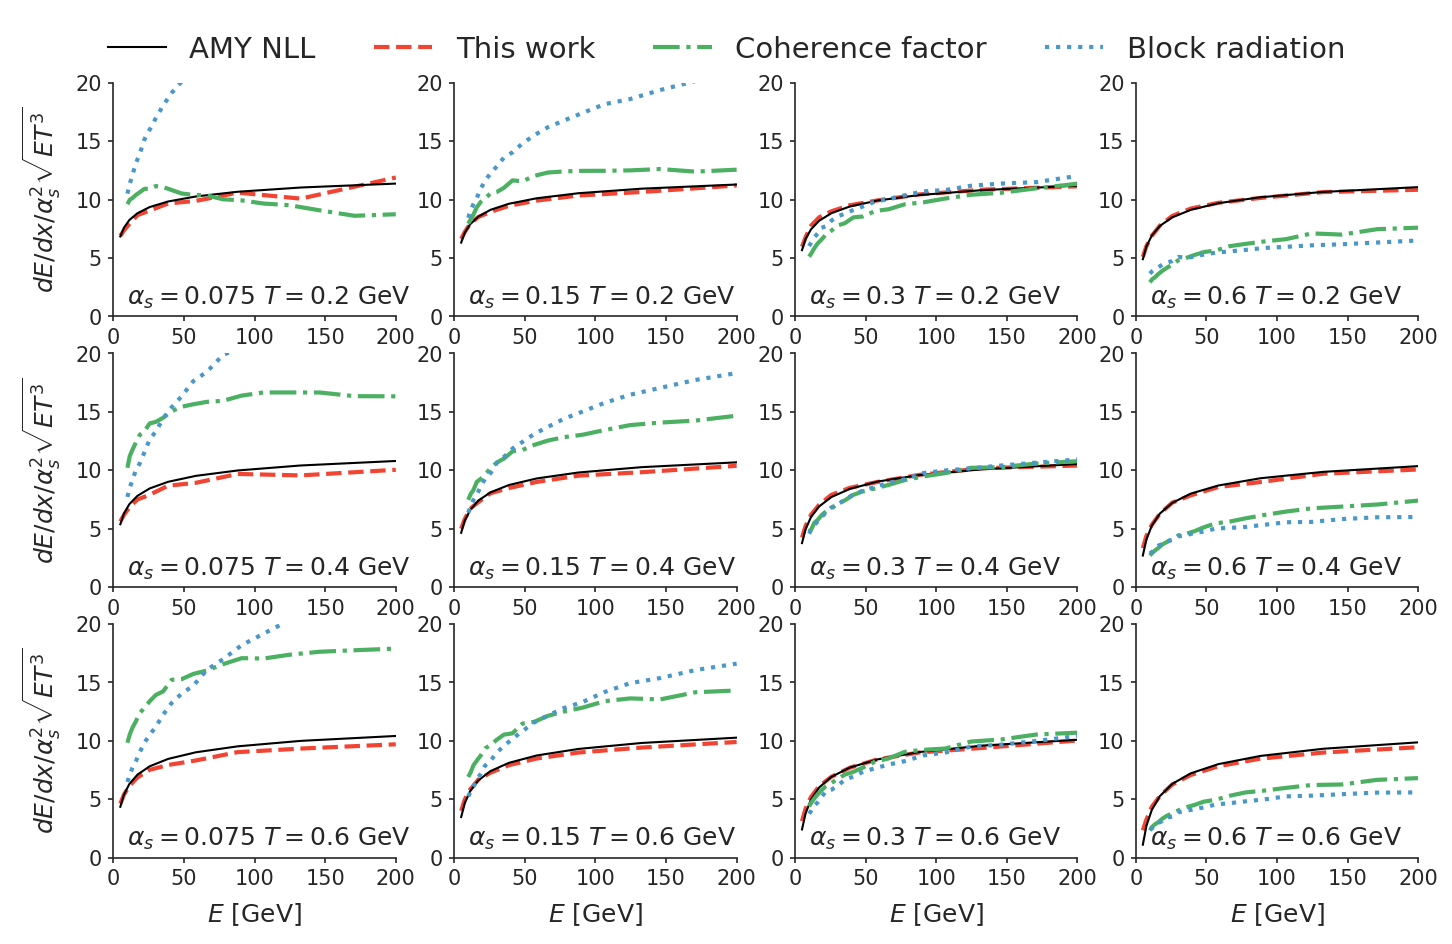
\includegraphics[width=1.\textwidth]{Eloss_infinite.png}
\caption[Energy loss per unit path length $dE/dx$ as a function of energy $E$,]{Energy loss per unit path length $dE/dx$ as a function of energy $E$, temperature $T$ and coupling constant $\alpha_s$. Each column corresponds to a value of the coupling constant $\alpha_s = 0.075, 0.15, 0.3$, and $0.6$ (from left to right). Each row corresponds to a temperature of $T = 0.2, 0.4$, and $0.6$ GeV (from top to bottom). $dE/dx$ is divided by the expected scaling $\alpha_s^2 \sqrt{ET^3}$. The MC implementations in this work (red dashed lines) is compared to the ``coherence factor'' approach (green dash-dotted lines) and the ``block radiation'' approach (blue dotted lines). The analytic results are denoted as black solid lines.}
\label{fig:eloss-inf}
\end{figure}

\begin{figure}
\singlespacing
\centering
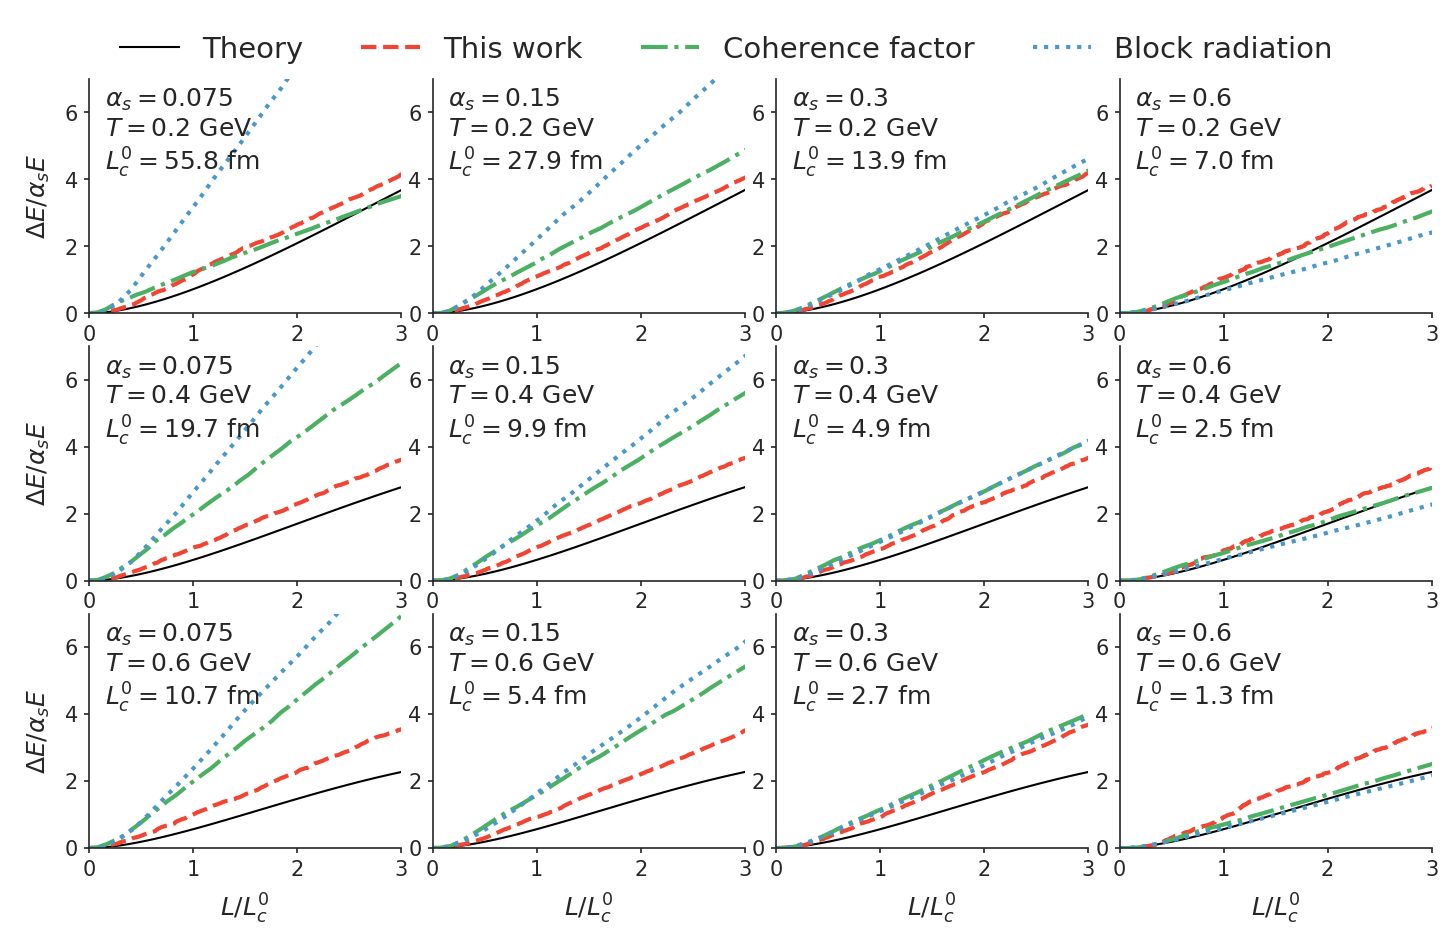
\includegraphics[width=1.\textwidth]{Eloss_Ldep.png}
\caption[Energy loss $\Delta E$ as a function of path length $L$, temperature $T$]{Energy loss $\Delta E$ as a function of path length $L$, temperature $T$ and coupling constant $\alpha_s$. Each column corresponds to a coupling constant of value $\alpha_s = 0.075, 0.15, 0.3$, and $0.6$ (from left to right). Each row corresponds to a temperature of value $T = 0.2, 0.4$, and $0.6$ GeV (from top to bottom). $\Delta E$ is scaled by $\alpha_s E$ and $L$ is scaled by an estimated critical path length $L_c^0 = \sqrt{E/\hat{q}_0}$, $\hat{q}_0 = C_A \alpha_s T m_D^2$. The MC implementations in this work (red dashed lines) is compared to the ``coherence factor'' approach (green dash-dotted lines) and the ``block radiation'' approach (blue dotted lines). The analytic results for a thin medium are denoted as black solid lines.}
\label{fig:eloss-ldep}
\end{figure}

\subsection{Energy loss comparison among the three approaches}
In Figure \ref{fig:eloss-inf}, we show the calculation of energy loss per unit path length $dE/dx$ of a quark in an ``infinitely large'' medium. 
Technically, $dE/dx$ is measured after an evolution time long enough ($L\gg L_c$) that finite size effects have faded away.
The results presented are normalized by $1/(\alpha_s^2 \sqrt{ET^3})$ in anticipation of the scaling $dE/dx \propto \alpha_s^2 \sqrt{ET^3}$.
For each column, we double the value of $\alpha_s$, and for each row, the temperature is increased by $0.2$ GeV. 
Within each subplot, the parton energy varies from $10$ GeV to $200$ GeV.
Different Monte Carlo implementations of the LPM effect are shown in colored lines, AMY NLL results are shown as black bands\footnote{\singlespacing we only integrate $\omega$ above the Debye mass to calculate the AMY energy loss}. 
Without a surprise, the ``modified approach'' approach (red-dashed lines) reproduces the energy, temperature, and coupling constant dependence of AMY NLL energy loss very well.
The ``coherence factor'' approach (blue-dash-dotted lines) has a similar energy and temperature dependence to that of the theoretical baseline; however, it systematically deviates from the baseline for different values of the coupling constant in a logarithmic manner.
For the ``block radiation'' approaches, the deviations from the baseline regarding their $\alpha_s$-dependence are even stronger, and the energy dependence also gets worse, which is not surprising as we have discussed its problems.

Next we examine the path-length ($L$) dependence of the energy loss $\Delta E$ of a quark with an initial energy of $E = 200$ GeV in a finite medium in Figure \ref{fig:eloss-ldep}.
Again, each column uses a different coupling constant, and each row uses a different temperature. 
The path length within each subplot is varied up to four times $L_c^0$.
Here $L_c^0 = \sqrt{E/\hat{q}_0}$ with $\hat{q}_0 = C_A \alpha_s T m_D^2$ estimating the critical path length below which one expects a clear non-linear path-length dependence.
All three implementations show the non-linear increase of $\Delta E$ as a function of $L$.
The ``modified Boltzmann'' approach stays close to the theory calculations when $L<L_c^0$ for all cases, while the other two methods deviate systematically as $\alpha_s$ is varied, similar to our previous findings for the energy-loss in the infinite matter case.

